\chapter{文件管理}\label{OS04}

\par\medskip\noindent\textbf{章节脉络}\par\smallskip
\begin{wideblock}\centering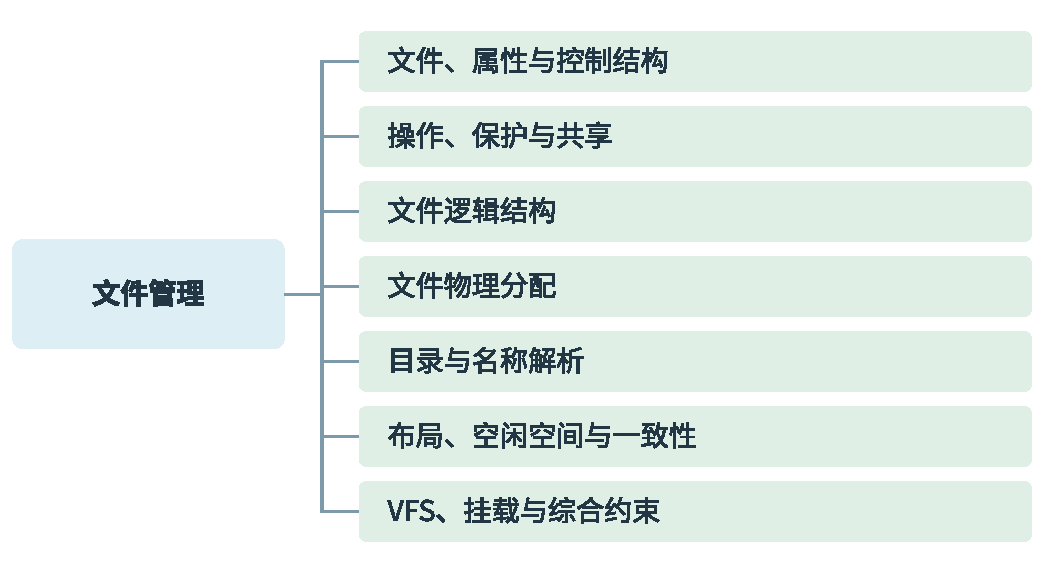
\includegraphics[width=\linewidth,height=92mm,keepaspectratio]{figures/overview.pdf}\end{wideblock}\par\medskip

\section{名称路径、数据路径与分配单位}\label{OS04-guide}

\begin{methodbox}[文件题先画四类节点]

\begin{enumerate}
\def\labelenumi{\arabic{enumi}.}
\tightlist
\item
  名称路径：根或当前目录，逐层目录项，以及解析出的inode。
\item
  使用关系：进程fd、打开实例、共享inode，标明位置指针属于哪一层。
\item
  数据路径：文件内偏移到逻辑块号，再经过直接或间接索引取得物理块号。
\item
  成本与容量：逐个扣除已缓存节点；分别计算数据块、索引块、inode和空闲管理的约束。
\end{enumerate}

\end{methodbox}

\begin{definition}[名称、文件本体和一次打开是三个对象]

目录项建立名字与文件标识的联系；inode保存文件本体的属性和块定位；打开实例保存这次使用的访问方式及当前位置，进程描述符再引用打开实例。三者的共享关系、计数与生命周期分别判断。

\end{definition}

\subsection{混合索引容量的逐层推导}\label{OS04-capacity-proof}

\begin{proof}[每增加一级索引，覆盖数乘一次扇出]

设块长为\(B\)字节，每个块号占\(e\)字节，一个纯索引块可容纳\(q=\lfloor B/e\rfloor\)个地址；inode有\(d\)个直接项和各一个一级、二级、三级间接项。直接区覆盖\(d\)个数据块；一级覆盖\(q\)个，二级覆盖\(q^2\)个，三级覆盖\(q^3\)个。因此理论用户数据上限为\((d+q+q^2+q^3)B\)。这要求相应地址字段可表示所需块号、所有分支可用，且未遇文件大小字段或卷容量等更紧上限；索引块开销另外计算。

\end{proof}

文件系统把``按名称找到数据''分成几步：由路径查目录项，由目录项找到文件控制信息，再把文件内偏移转换成存储块位置。目录、索引节点、打开文件表和数据块分别承担不同工作；把它们笼统当成``文件的信息''，就会把访问次数算混。

本章文件内字节偏移和逻辑块号从 0 开始；``第几个记录''若采用自然序号则从 1 开始。除题目另有定义，1 KB 为 1024 B。计算访盘次数时，要逐次说明所访问的目录块、索引块或数据块中哪些尚不在内存；已缓存的内容不重复计入。

\section{文件、文件控制块与索引节点}\label{OS04-6-1}

\textbf{文件}是具有名称和一定属性的持久数据集合。从使用者看，它可以是字节流，也可以由记录组成；从存储看，它最终占据若干物理块。文件的名称与内容不是同一个对象，一个文件可以通过多个名称被访问。

\textbf{文件控制块 FCB}是系统描述和管理文件的数据结构，通常记录类型、大小、所有者、权限、时间和存储位置等元数据。将文件名与其他描述信息分离时，目录项可只保留``文件名---索引节点号''，其余信息由\textbf{索引节点 inode}保存。inode 是这种设计中的文件控制信息载体，不是文件数据块，也不只是``指向文件的一个指针''。

索引节点号的意义局限于相应文件系统，不能只凭两个分区上的编号相同就判断是同一个文件。内存中的 inode 还可包含运行时锁、引用计数等；它与磁盘中持久保存的 inode 相关，但字段不必完全相同。

目录本身也是文件，其中存放的是用于查找对象的目录项；普通文件的名字出现在目录中，数据内容并不因此存入目录。采用 inode 的模型还应区分三个位置：名字在目录项中，属性和块地址在 inode 中，用户内容在数据块中。

\begin{wideblock}

\par\medskip\noindent\begin{minipage}{\linewidth}\fontsize{9.3}{12}\selectfont\begin{tabularx}{\linewidth}{@{}YYYY@{}}
\toprule\noalign{}
\begin{minipage}[b]{\linewidth}\raggedright
对象
\end{minipage} & \begin{minipage}[b]{\linewidth}\raggedright
记录什么
\end{minipage} & \begin{minipage}[b]{\linewidth}\raggedright
由什么找到它
\end{minipage} & \begin{minipage}[b]{\linewidth}\raggedright
何时改变或回收
\end{minipage} \\
\midrule\noalign{}


目录项 & 当前目录内的名字及 inode 号 & 逐层解析路径、查找所在目录 & 建立、重命名、增删链接时改变；关闭文件不删除它 \\
磁盘 inode & 文件类型、大小、权限、链接数、数据块地址等持久信息 & 在本文件系统解释 inode 号 & 文件内容或属性改变时更新；须满足无链接、无有效使用引用等回收条件 \\
内存 inode & 已载入的文件信息及运行时锁、引用状态等 & inode 缓存或打开对象引用 & 可由多个打开者共享；无打开者后是否立即释放取决于缓存模型 \\
打开实例与进程描述符表 & 打开实例记录文件位置、访问方式；进程表把 fd 关联到实例 & 已返回的 fd 在所属进程内解释 & open 建立，dup 或继承可共享实例，close 释放相应引用 \\
\bottomrule\end{tabularx}
\end{minipage}\par\medskip

\end{wideblock}

因此``知道文件名''``知道 inode 号''``inode 已在内存''和``数据已缓存''依次消除了不同查找步骤。访盘题要把题设明确命中（已在内存）的对象从访问路径中扣除，不能由其中一个条件推得其他对象也都在内存。

\section{建立、打开、读写、关闭与删除}\label{OS04-6-2}

\textbf{建立文件}要分配文件控制信息，在父目录增加名字与文件标识的关联，并按规则初始化属性；空文件可以暂不分配实际数据块。\textbf{打开文件}按路径查找、检查权限，在内存建立或引用打开状态，返回文件描述符。打开不等于把整个文件内容读入内存。

一个常用抽象分为三层：进程文件描述符表把小整数 \texttt{fd} 指向打开实例；打开实例保存本次打开的状态，例如当前文件位置和访问方式；内存 inode 保存文件本身的共享属性及定位信息。不同教材有时把后两层合称系统打开文件表，本书计算前会说明各字段属于哪一层，避免因表名不同把状态混在一起。

\subsection{课件示例：打开目录 M 中的文件 A}\label{OS04-course-open}

课件模型中，外存目录 M 含 \texttt{FCB\_A}、\texttt{FCB\_B}、\texttt{FCB\_C}、\texttt{FCB\_D}，最近访问的目录项也可缓存在内存。调用 \texttt{open(\allowbreak{}.\allowbreak{}.\allowbreak{}.\allowbreak{}/\allowbreak{}M/\allowbreak{}A,\allowbreak{} 只读)\allowbreak{}} 时，系统沿路径查找并读入必要目录，找到 A 的目录项，建立或引用系统打开文件表项，再为调用进程建立表项并返回描述符。

\begin{wideblock}

\par\medskip\noindent\begin{minipage}{\linewidth}
\centering
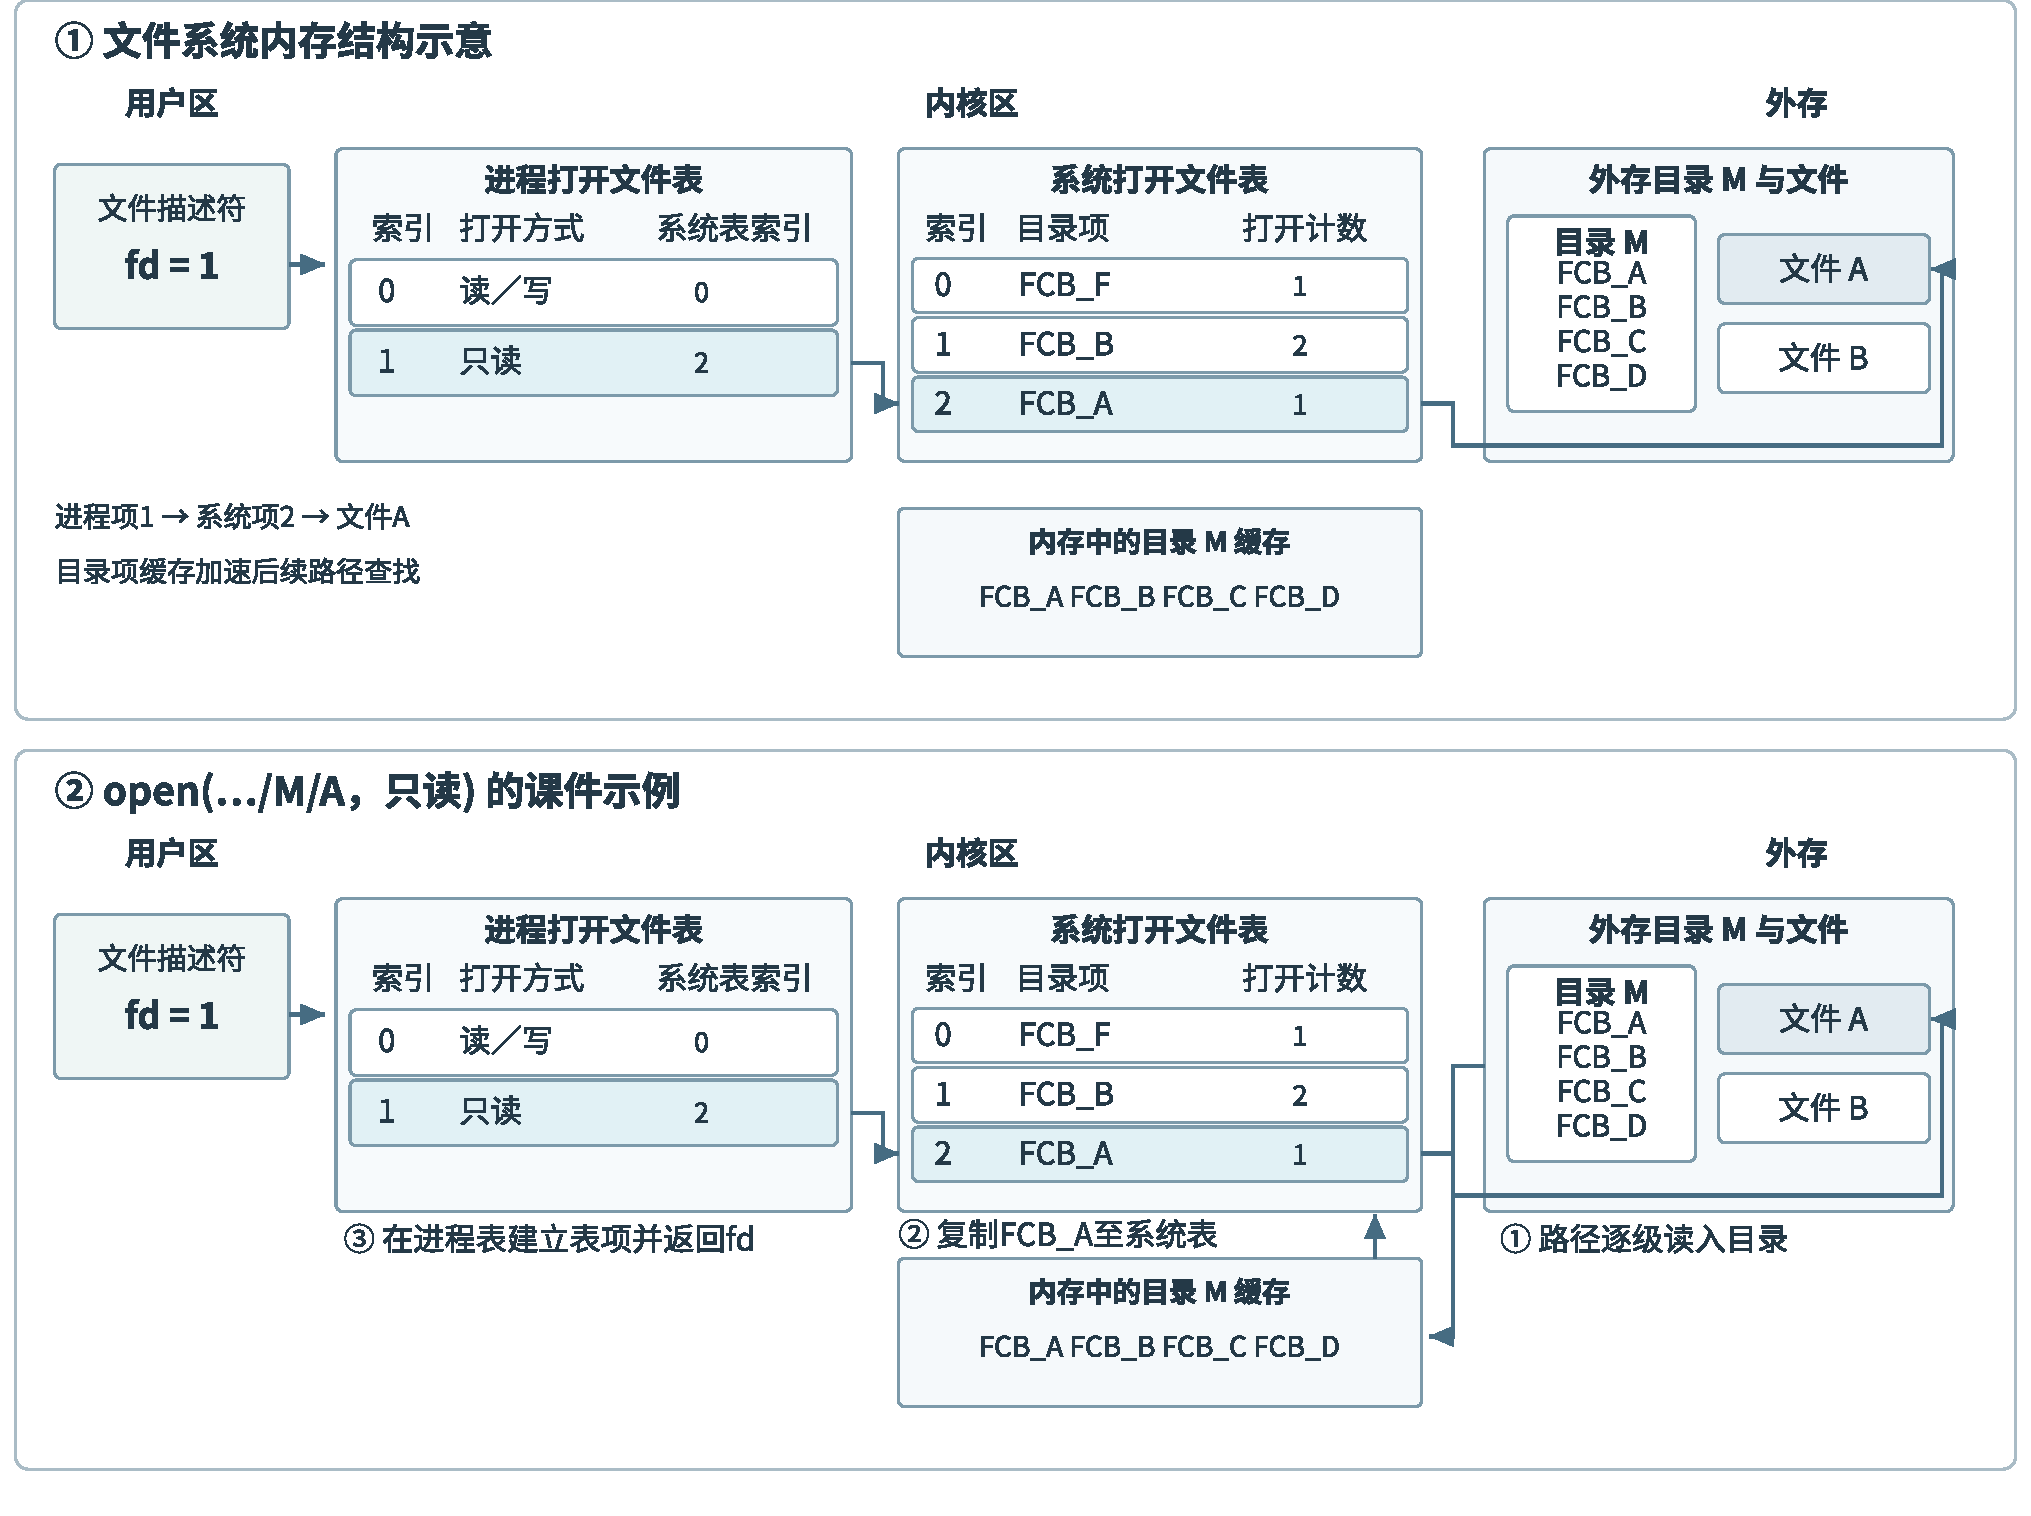
\includegraphics[width=\linewidth,height=125mm,keepaspectratio]{figures/OS_open_course.pdf}
\captionof{figure}{课件中的目录缓存、进程打开表、系统打开表及文件 A 的打开路径}\label{os-fig-open-course}
\end{minipage}\par\medskip

\end{wideblock}

图中进程打开表的 1 号项以只读方式指向系统表的 2 号项；系统项 2 是 \texttt{FCB\_A}，打开计数为 1，返回 \texttt{fd=\allowbreak{}1}。同一系统表还有 \texttt{FCB\_F}、\texttt{FCB\_B} 两项，其打开计数分别为 1 和 2；这两个数字用于示例中各表项的引用关系，不能看成 A 的硬链接数。目录缓存是名称查找的加速结构，打开文件表管理已经打开的对象，两者职责不同。

\texttt{read(\allowbreak{}fd,\allowbreak{}buf,\allowbreak{}n)\allowbreak{}} 根据打开状态和当前偏移找到目标数据，必要时发起 I/O，向用户区返回实际读到的字节，并更新相应文件位置。\texttt{write} 可能分配新块、改变大小、把缓存标记为脏；返回成功不必表示数据已立即持久化到盘片。文件结束、短读、权限错误等应按题给语义处理。

\textbf{关闭}释放本次打开引用，必要时更新元数据；它不等于删除文件。\textbf{删除名字}从目录取消关联，硬链接计数随之变化；文件内容何时真正回收，还要检查是否仍有其他硬链接或有效打开引用。两类计数含义不同：磁盘硬链接数统计名字关联，打开引用数统计运行中的使用关系。

\subsection{例 4-1　最后关闭，释放的是哪一层}\label{OS04-ex6-1}

\begin{example}[配套例题]

【配套例题】 若文件 F 仅被进程 P 打开并访问，则当进程 P 关闭 F 时，文件系统需要完成的是（　）。

A. 删除目录文件中 F 的目录项

B. 释放 F 的索引节点所占的内存空间

C. 释放 F 的索引节点所占的外存空间

D. 将文件磁盘索引节点中的链接计数减 1

\end{example}

\textbf{解析。} 本题按``最后关闭时释放相应内存控制信息''的简化模型处理，答案为 \textbf{B}。A、C 属于删除持久对象的工作，D 对应硬链接关系改变；关闭并不取消文件名。实际系统可以把暂时没有打开者的 inode 留在缓存里，缓存回收时机与本题抽象不同，不能据此把 close 与 unlink 混为一谈。

\subsection{文件位置可以共享，也可以独立}\label{OS04-auto-1}

两个进程分别 \texttt{open} 同一文件，通常得到两个打开实例，各有自己的文件位置，但都指向同一文件的 inode。通过 \texttt{dup} 或进程继承共享同一打开实例时，文件位置也可能共享。因此``同一个文件''不决定读写位置是否相同；先看是否同一次打开的引用。

多个进程以写方式打开同一文件，不表示文件系统自动满足应用所需的完整事务互斥。要防止记录被交错修改，应使用规定的锁或其他同步方式。系统对单次写的原子性规则也不能任意推广为整个``读---修改---写''序列的原子性。

\subsection{课件示例：两个进程打开同一文件}\label{OS04-course-shared-open}

课件的抽象模型把每个进程的读写指针、访问权限放在各自的进程打开表中，把文件及其打开计数放在系统打开表中。进程 A 的 2 号表项以只读方式打开 \texttt{test.\allowbreak{}txt}，进程 B 的 1 号表项以读写方式打开同一文件；两个表项均指向系统表的 \texttt{k} 号表项，系统表所示打开计数为 2。

\begin{wideblock}

\par\medskip\noindent\begin{minipage}{\linewidth}
\centering
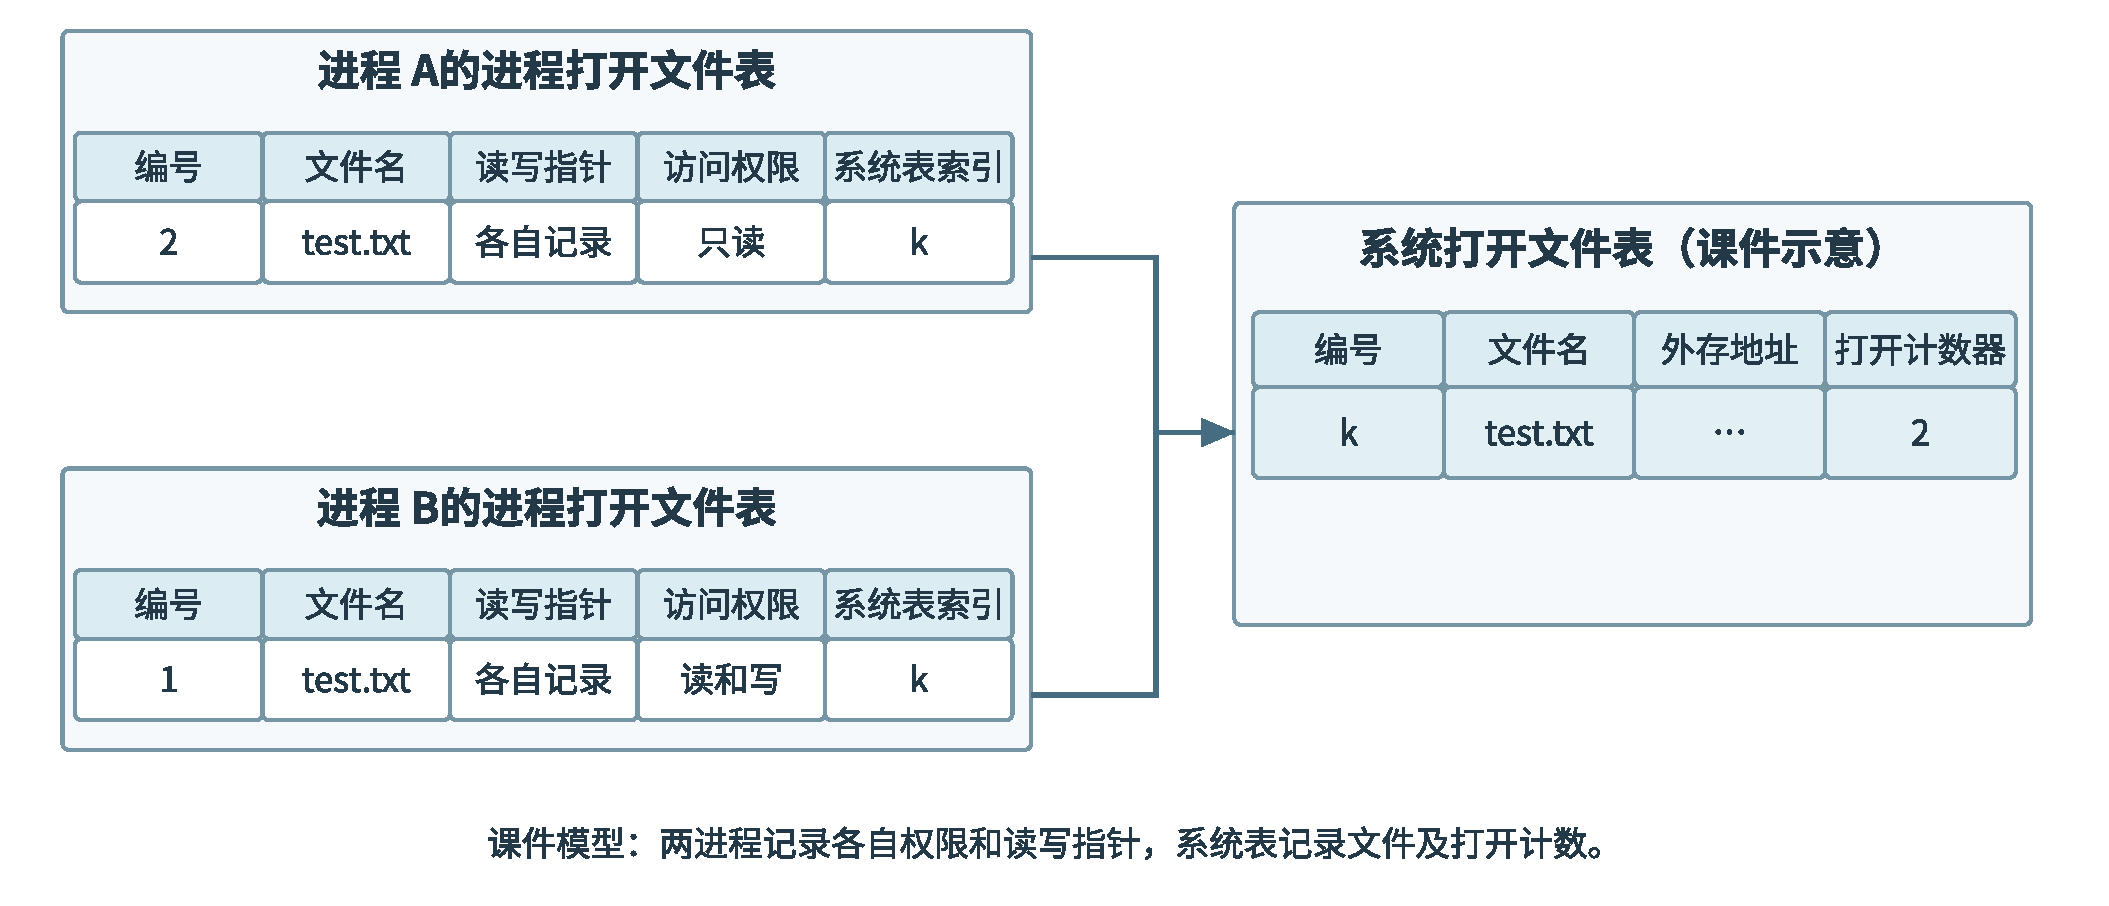
\includegraphics[width=\linewidth,height=125mm,keepaspectratio]{figures/OS_shared_open_course.pdf}
\captionof{figure}{两个进程的打开文件表指向系统表中同一文件项，打开计数为2}\label{os-fig-shared-open-course}
\end{minipage}\par\medskip

\end{wideblock}

这一课件示例中，两进程的读写指针和权限各自记录。它与前面把偏移存于``打开实例''的模型采用了不同的表项划分：对具体系统要先确定表项代表共享文件信息还是一次打开，再判断偏移是否共享；同一个文件身份本身并不决定两次使用是否共享偏移。系统表中的打开计数也不能当作磁盘 inode 的硬链接数。

\section{文件保护：用户类别与权限组合}\label{OS04-6-3}

保护回答谁能对对象执行什么操作。口令、加密和访问控制各有作用，不能相互替代：加密保护内容不被未授权读取，访问控制由系统按身份与权限限制操作；读权限、写权限、执行权限也不同于调度优先级。

访问矩阵以主体为行、对象为列，格中保存允许操作集合。按对象列存放形成访问控制表 ACL，便于查``谁能使用这个文件''；按主体行组织授权可形成能力表一类机制，便于查``这个主体能用哪些对象''。保护还涉及授权、撤销和检查时机；权限存进去之后，访问时仍须逐次检查。

课件以一个文件的访问控制表说明：1表示该用户允许对应操作，0表示不允许。此表记录的是各主体针对同一文件的权限，并非文件内容本身。

\begin{wideblock}\par\medskip\noindent\begin{minipage}{\linewidth}\fontsize{9.3}{12}\selectfont\begin{tabularx}{\linewidth}{@{}YYYYYYY@{}}
\toprule\noalign{}
用户 & 读 & 写 & 执行 & 添加 & 删除 & 列表清单 \\
\midrule\noalign{}


father & 1 & 1 & 1 & 1 & 1 & 1 \\
mother & 1 & 0 & 1 & 0 & 0 & 1 \\
son & 0 & 0 & 0 & 0 & 0 & 0 \\
\bottomrule\end{tabularx}
\end{minipage}\par\medskip\end{wideblock}

例如mother可以读取或执行，但表中未授予写入、追加和删除。若用户很多，可以按组记录权限；课件的另一示例中，系统管理员拥有五项权限，文件主拥有执行、修改、读取和写入，文件主的伙伴拥有执行和读取，其他用户均未被授予这些权限。访问时仍须先确定主体所属组，再按表和系统冲突处理规则检查。

\subsection{例 4-2　权限可以同时成立，不能只编码一种}\label{OS04-ex6-2}

\begin{example}[配套例题]

【配套例题】 某文件系统针对每个文件，把用户分成安全管理员、文件主、文件主的伙伴、其他用户 4 类；访问权限有完全控制、执行、修改、读取、写入 5 种。若 FCB 中用二进制位串表示不同类别用户对一个文件的访问权限，至少需要多少位？

A. 5　　B. 9　　C. 12　　D. 20

\end{example}

\textbf{解析。} 对一类用户，五种权限可分别有或没有，需要 5 个独立二进制位。四类用户分别保存其权限组合，需要 \(4\times5=20\) 位，答案为 \textbf{D}。用 2 位编码用户类别、3 位编码一种操作，只能表达``是哪一类、做哪一种''，不能同时记录四类用户各自的权限组合。题目未给权限之间必然蕴含关系，因此不能因``完全控制''这个名称擅自压缩其他位。

\subsection{口令、加密与权限表的具体差别}\label{OS04-protection-methods}

课件的口令模型为每个文件保存验证信息，用户提交正确口令后才可访问。其空间和比较开销较小，但口令的保管、共享和泄露会影响保护效果。实际系统可以保存校验结果而不是明文口令，具体格式由系统规定。

加密将可读明文转换成密文，解密需要正确的密钥。课件用异或说明可逆性：明文\texttt{00101011000111010001}，重复使用密钥\texttt{01001}，得到密文\texttt{01100001010011111000}；再次用同一重复密钥异或恢复明文。若采用另一密钥\texttt{01111}，则不能还原同一内容。这里展示的是异或的代数过程，不能据此把这一简单重复密钥方案等同于现代保密系统。

权限表控制某主体被允许执行的操作，口令验证身份或访问凭证，加密保护数据的可读性，三者可以配合。精简ACL将用户分组，记录各组的操作位，再在访问时确定用户所属组。目录的查找、列出与修改权限还影响能否到达下级名字；目录权限与文件内容权限应按各自操作检查，不能仅凭``目录允许访问''推断所有文件均可读写。

课件还用精简 ACL 演示分组授权：表中 1 表示允许该项操作，0 表示不允许；系统据用户所属组检查相应权限。

\begin{wideblock}\par\medskip\noindent\begin{minipage}{\linewidth}\fontsize{9.3}{12}\selectfont\begin{tabularx}{\linewidth}{@{}YYYYYY@{}}
\toprule\noalign{}
用户组 & 完全控制 & 执行 & 修改 & 读取 & 写入 \\
\midrule\noalign{}


系统管理员 & 1 & 1 & 1 & 1 & 1 \\
文件主 & 0 & 1 & 1 & 1 & 1 \\
文件主的伙伴 & 0 & 1 & 0 & 1 & 0 \\
其他用户 & 0 & 0 & 0 & 0 & 0 \\
\bottomrule\end{tabularx}
\end{minipage}\par\medskip\end{wideblock}

例如，将用户加入``文件主的伙伴''组后，该用户在此课件模型中具有执行和读取权限。此表是演示用权限配置；实际系统中的组成员关系、权限继承与拒绝规则须按具体机制判断。

\subsection{课件示例：Windows文件夹访问控制}\label{OS04-windows-acl-demo}

课件以文件夹\texttt{E:\allowbreak{}\textbackslash{}照片}和名为``临时访客''的本地账户演示访问控制。主要关系如下：

\par\medskip\noindent\begin{minipage}{\linewidth}\fontsize{9.3}{12}\selectfont\begin{tabularx}{\linewidth}{@{}YY@{}}
\toprule\noalign{}
\begin{minipage}[b]{\linewidth}\raggedright
步骤
\end{minipage} & \begin{minipage}[b]{\linewidth}\raggedright
课件中的操作或现象
\end{minipage} \\
\midrule\noalign{}


准备主体 & 创建``临时访客''本地账户，作为需要限制访问的用户 \\
选择对象 & 打开\texttt{E:\allowbreak{}\textbackslash{}照片}的属性，在``安全''设置中查看该文件夹的用户、组与权限 \\
建立规则 & 把``临时访客''加入权限设置，对选定权限在``拒绝''列勾选 \\
系统提示 & Windows提示：若用户所属的两个组对同一权限分别允许和拒绝，拒绝项会优先于允许项 \\
验证结果 & 切换到``临时访客''尝试打开该文件夹，课件示例显示当前用户无权访问 \\
\bottomrule\end{tabularx}
\end{minipage}\par\medskip

这个例子把主体、对象和权限明确对应起来。显示的界面与具体用户组是课件运行环境的实例；实际有效权限还要按系统规则检查适用的显式条目、继承条目和用户所属组，不能仅凭一项允许就断定一定可访问。

\section{逻辑结构：字节流和记录怎样被使用}\label{OS04-6-4}

\textbf{无结构文件}向应用提供字节序列，记录边界由应用自行解释；所谓无结构不是没有字节顺序。\textbf{有结构文件}由记录组成，可以定长或变长。定长记录且不跨块时，记录位置容易由长度计算；变长记录需要额外的边界、长度或索引信息。

顺序文件按记录次序存放，适合顺序处理；按关键字组织的顺序文件可利用有序性查找，但插入维护可能较贵。索引文件为记录或记录组维护索引，便于定位；索引顺序文件把顺序组织与索引结合。这些是应用看到的、或逻辑层规定的记录组织；它们与下面讲的物理块分配（连续、链接、索引）不是同一维度。

例如变长记录文件可以用一个逻辑索引定位记录所在字节范围，文件本身再通过物理索引块定位磁盘块。两个``索引''服务不同层次，题目问哪个对象的空间、哪个访问链，就沿对应关系计算。

\subsection{顺序文件的串结构与顺序结构}\label{OS04-sequential-records}

顺序文件中的记录按逻辑次序排列。若记录间按存入的先后关系排列，称为\textbf{串结构}；若按关键字的顺序排列，称为\textbf{顺序结构}。这里的``串''不是把记录强制变为字符，也不规定其底层磁盘分配方式。

给定第0条记录的逻辑地址\(F\)，定长记录长度为\(L\)，若记录在逻辑文件中连续排列，则第\(i\)条记录起址为\(F+iL\)，因此支持按记录号直接定位。若记录变长，必须先知道前面记录的长度或另设索引；即使是定长记录，若逻辑记录通过链接组织，也通常要沿链接查找。

``按记录号找第\(i\)条''与``按关键字找某个人''是两个问题。定长、连续布局解决前者；再按关键字有序，才可利用有序性做折半等检索。串结构中的关键字一般只能顺序查找。增删时也要分别维护记录布局和关键字次序。

\subsection{索引文件与索引顺序文件怎样折中}\label{OS04-record-index}

\textbf{索引文件}为记录建立定长索引项，如``关键字、记录长度、记录逻辑地址''。索引项连续且定长，定位第\(i\)个索引项容易，再沿其地址找到可变长记录。不同数据项可各建索引，例如学号索引与姓名索引；新增、删除或修改记录时，相关索引也要保持一致。

每记录一项会有空间代价：若记录平均8 B、索引项32 B，索引本身是原记录数据的4倍。\textbf{索引顺序文件}改为一组记录对应一个索引项，先定位组再在组内顺序查找；组与组之间要有能用于定位的关系，组内可按课件模型无需关键字有序。

\par\medskip\noindent\begin{minipage}{\linewidth}
\centering
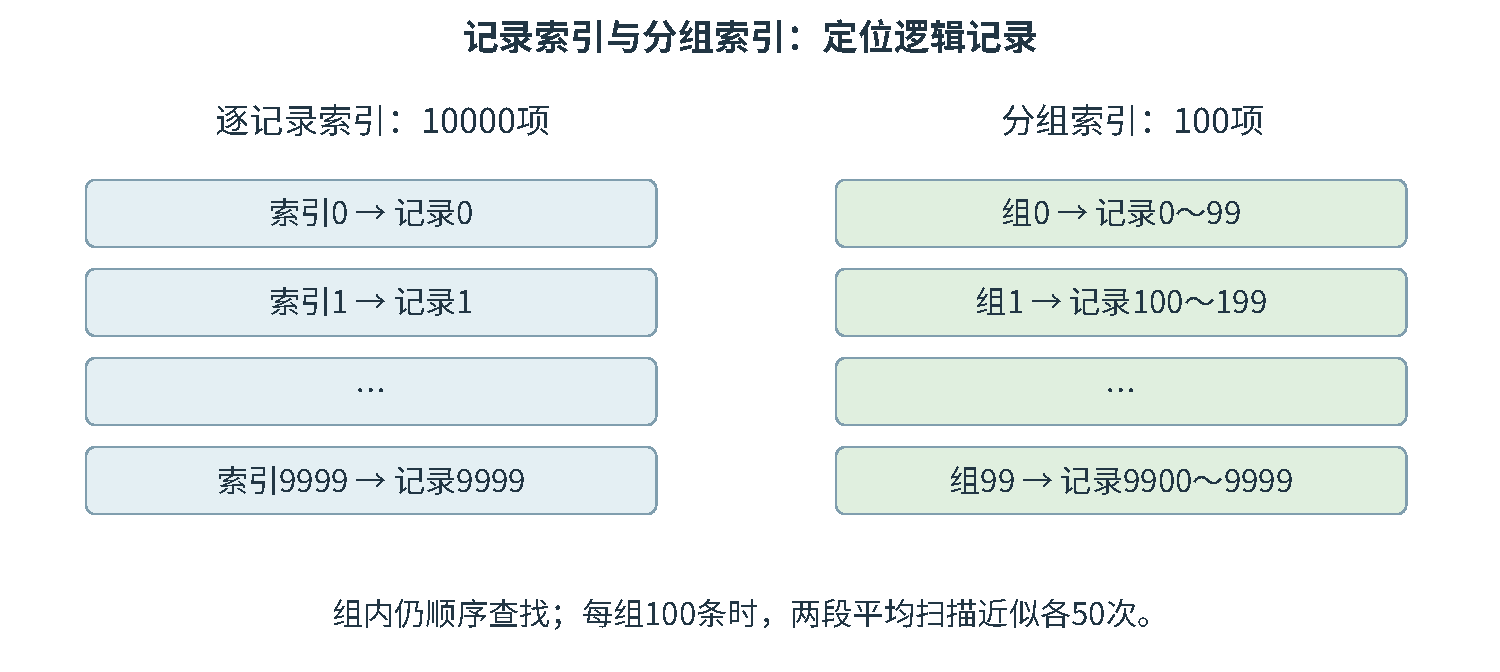
\includegraphics[width=\linewidth,height=125mm,keepaspectratio]{figures/OS_record_indexes.pdf}
\captionof{figure}{逐记录索引与分组索引的目标不同，索引保存记录的逻辑地址}\label{os-fig-record-index}
\end{minipage}\par\medskip

课件例有10000条记录，按100组、每组100条组织。顺序扫描组索引与组内记录，平均比较数近似为\(100/2+100/2=100\)，相对直接扫描10000条的约5000次明显减少。若严格假定成功位置等概率、各层都用包含成功比较的线性扫描，精确期望是\(50.5+50.5=101\)；``一半''是大规模近似口径。

一般地，\(N\)条记录分成\(g\)组，平均比较数近似为\(g/2+N/(2g)\)，在\(g\approx\sqrt N\)时两项平衡。若为\(10^6\)条记录建立两级索引，按每级100项分组，则顶级100项、低级共10000项、数据1000000条，查找需经过顶级、低级、组内三个100项的顺序扫描，近似\(50+50+50=150\)次，等概率精确值为151.5次。更一般的\(k\)级索引，等规模分组为\(N^{1/(k+1)}\)项，近似比较数为\((k+1)N^{1/(k+1)}/2\)。

这些比较数属于给定的线性扫描模型。若索引层改用折半或树结构，应按新的检索方法计算，不能继续沿用各层一半的公式。

\subsection{用户记录组织与系统块分配各解决哪一步}\label{OS04-two-mappings}

以每条记录64 B、每磁盘块1024 B为例：用户按记录号\(i\)得到逻辑字节偏移\(64i\)，所以逻辑块号为\(\lfloor i/16\rfloor\)，块内偏移为\((i\bmod16)64\)。接下来才由文件系统将逻辑块号映射为物理块号。

用户自建的记录索引映射“关键字\ensuremath{\to}记录逻辑地址”；文件系统的块索引映射“逻辑块号\ensuremath{\to}物理块号”。因此索引文件可以采用连续、链接或索引分配，顺序文件也可以采用这些物理分配方式。某一层支持直接定位，不自动保证另一层也只有一次访问。

\subsection{课件示例：记录组织与磁盘块组织}\label{OS04-course-record-layers}

同一份顺序文件的记录可以连续排列，也可以由用户设计的链接组织。课件示意中，学生0、1、2、3分别位于记录存储槽0、3、2、5，链接次序为\texttt{0 → 3 → 2 → 5}；记录间的链接先解决``下一个记录在哪''。在文件系统层面，文件被划分成逻辑块；这些逻辑块可另行采用连续分配或链接分配。因此，即使某种物理分配支持直接找到给定逻辑块，链式记录仍不一定能直接算出第\(i\)条记录的位置。

\begin{wideblock}

\par\medskip\noindent\begin{minipage}{\linewidth}
\centering
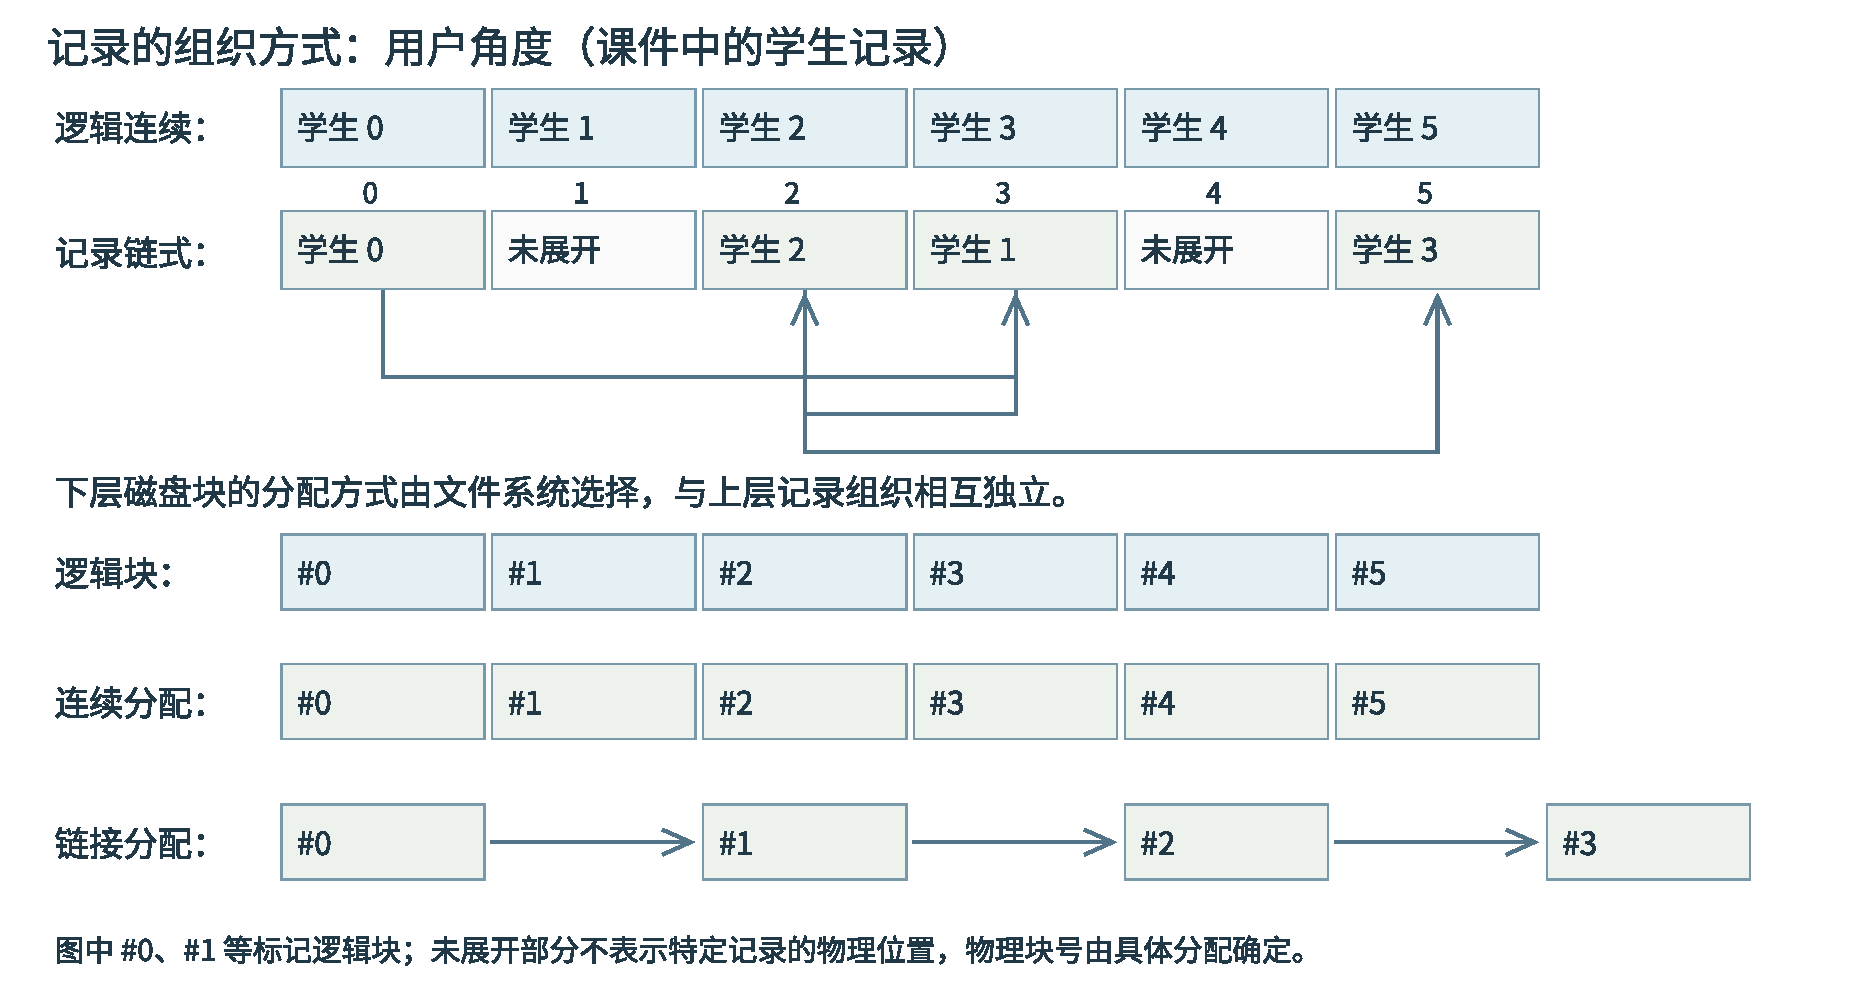
\includegraphics[width=\linewidth,height=125mm,keepaspectratio]{figures/OS_record_layers_course.pdf}
\captionof{figure}{学生记录的连续和链式组织，与文件逻辑块的连续和链接分配是两层独立关系}\label{os-fig-record-layers-course}
\end{minipage}\par\medskip

\end{wideblock}

课件以学生记录给出一个按记录号读取的实例，字段定义为\texttt{number}、\texttt{name[\allowbreak{}30]\allowbreak{}}、\texttt{major[\allowbreak{}30]\allowbreak{}}；在课件平台的\texttt{int}为4 B、结构体大小为64 B时，编号5的记录从逻辑偏移\(5\times64=320\) B开始。以下保留课件的记录类型与\texttt{fseek}／\texttt{fread}接口，并检查返回值：

\par\medskip\noindent\begin{minipage}{\linewidth}
\BlueLines{11,13,17}
\begin{codeblock}[language=C]
#include <stdio.h>

typedef struct {
    int number;
    char name[30];
    char major[30];
} Student_info;

int main(void) {
    FILE *fp = fopen("students.info", "rb");
    if (fp == NULL) return 1;
    Student_info stu;
    if (fseek(fp, 5L * sizeof(Student_info), SEEK_SET) == 0 &&
        fread(&stu, sizeof(Student_info), 1, fp) == 1)
        printf("学生编号：%d\n", stu.number);
    fclose(fp);
    return 0;
}
\end{codeblock}
\end{minipage}\par\medskip

这里假定文件按同一实现写入、至少有6条完整记录；\texttt{sizeof(\allowbreak{}Student\_info)\allowbreak{}}依赖平台的整型宽度与结构体对齐，64 B是课件平台的具体结果。课件演示使用\texttt{"r"}／\texttt{"w"}模式；读写原始结构体时使用\texttt{"rb"}／\texttt{"wb"}可以避免某些平台的文本模式转换。\texttt{fseek}指定文件中的逻辑位置，随后系统按文件分配方式完成逻辑块到物理块的转换；读取是否实际触发磁盘I/O，还受缓冲与缓存状态影响。

课件的无结构文件示例将\texttt{"Hello world!"}重复写入10000次。若每字符一字节、内容没有额外换行，文件长\(12\times10000=120000\) B；从0起编号的第16个字符在每12字节循环中的位置为\(16\bmod12=4\)，是\texttt{o}。\texttt{fgetc}读取一个字符时可经标准I/O缓冲，因而一次库函数调用不必然对应一次底层读系统调用。

\section{物理分配：连续、链接与索引}\label{OS04-6-5}

\textbf{连续分配}记录起始块与长度，逻辑块 \(k\) 直接映射为起始块加 \(k\)，顺序和随机访问都容易；但文件增长可能受相邻空间限制，空闲空间也可能有外部碎片。按区段扩展可缓解增长问题，但不是每个文件永远只有一个连续区间。

\textbf{隐式链接分配}在各数据块内保存后继块号，目录记录首块等信息。逻辑上连续的数据可散在任意物理块；增长容易、无需一个大连续洞，但要找后面的块通常必须沿链读取，链指针也占用空间。损坏一个指针会影响后续定位。

\textbf{显式链接分配}把后继关系集中到文件分配表 FAT。表若驻留内存，沿链查找不必每步读取数据块，但定位第 \(k\) 个簇仍要执行链追踪，不等于具有直接随机下标。FAT 一般为每个受管簇保存一项，规模取决于受管卷的簇数；不能仅凭某个文件的最大长度推断整个卷的 FAT 大小，除非题目另外限定了两者的关系。

\textbf{索引分配}为文件记录各逻辑块的物理块号，可单级、多级或混合索引。根据逻辑块号查相应索引项即可定位，支持随机访问；索引本身占空间，小文件使用大索引块时可能浪费。UNIX 式混合索引让小文件直接索引，大文件逐渐使用间接层级。

比较访盘次数时，先统一起点：逻辑块号 \(k\) 从 0 开始，目录项或 inode 已在内存，查找路径上的数据块和索引块均未缓存，也没有预存的中间块号；FAT 行另假定分配表已驻留内存。

\begin{wideblock}

\par\medskip\noindent\begin{minipage}{\linewidth}\fontsize{9.3}{12}\selectfont\begin{tabularx}{\linewidth}{@{}YYYY@{}}
\toprule\noalign{}
\begin{minipage}[b]{\linewidth}\raggedright
分配方式
\end{minipage} & \begin{minipage}[b]{\linewidth}\raggedright
怎样定位第 \(k\) 个逻辑块
\end{minipage} & \begin{minipage}[b]{\linewidth}\raggedright
读取目标块需访盘
\end{minipage} & \begin{minipage}[b]{\linewidth}\raggedright
额外组织空间
\end{minipage} \\
\midrule\noalign{}


连续 & 起始块号加 \(k\)，可直接定位 & 1次 & 起始块号、长度等描述信息 \\
隐式链接 & 从首块读取后继指针，逐块追踪 & \(k+1\) 次 & 数据块中的后继指针 \\
显式链接 FAT & 在内存表中追踪 \(k\) 条链接，再读目标块 & 1次，但仍有内存追链开销 & 全卷每簇的表项；驻留表占内存 \\
单级、多级或混合索引 & 按块号确定索引项，逐级取得下层块号 & 经 \(h\) 级间接索引时 \(h+1\) 次；直接指针为1次 & 文件的索引项和索引块 \\
\bottomrule\end{tabularx}
\end{minipage}\par\medskip

\end{wideblock}

\begin{wideblock}

\par\medskip\noindent\begin{minipage}{\linewidth}\fontsize{9.3}{12}\selectfont\begin{tabularx}{\linewidth}{@{}YY@{}}
\toprule\noalign{}
分配方式 & 增长与碎片 \\
\midrule\noalign{}


连续 & 扩展受相邻空间制约；可能有外部碎片 \\
隐式链接 & 可离散追加；无外部碎片 \\
显式链接 FAT & 可离散追加；受空闲簇及表规模约束 \\
单级、多级或混合索引 & 可离散追加；范围受各级索引容量限制 \\
\bottomrule\end{tabularx}
\end{minipage}\par\medskip

\end{wideblock}

FAT 支持不读取前面数据块而访问指定块，这正是它相对隐式链接的优势；这不表示由块号定位物理块只需常数次内存访问。``无外部碎片''也不表示最后一个数据块一定装满，各方式仍可能留下块内未用空间。题目改变 inode、FAT 或索引块的缓存条件时，先删去已命中的那一级访问，再计总数。

\subsection{例 4-3　混合索引中，一次访问要经过几层}\label{OS04-ex6-3}

\begin{example}[配套例题]

【配套例题】 文件索引节点中有 10 个直接索引指针，一级和二级索引指针各 1 个。磁盘块为 1 KB，每个索引指针 4 B。某文件索引节点已在内存，把该文件偏移量为 1234 和 307400（按字节编址）处所在的磁盘块读入内存，需要访问的磁盘块个数分别是（　）。

A. 1、2　　B. 1、3　　C. 2、3　　D. 2、4

\par\medskip\noindent\begin{minipage}{\linewidth}
\centering
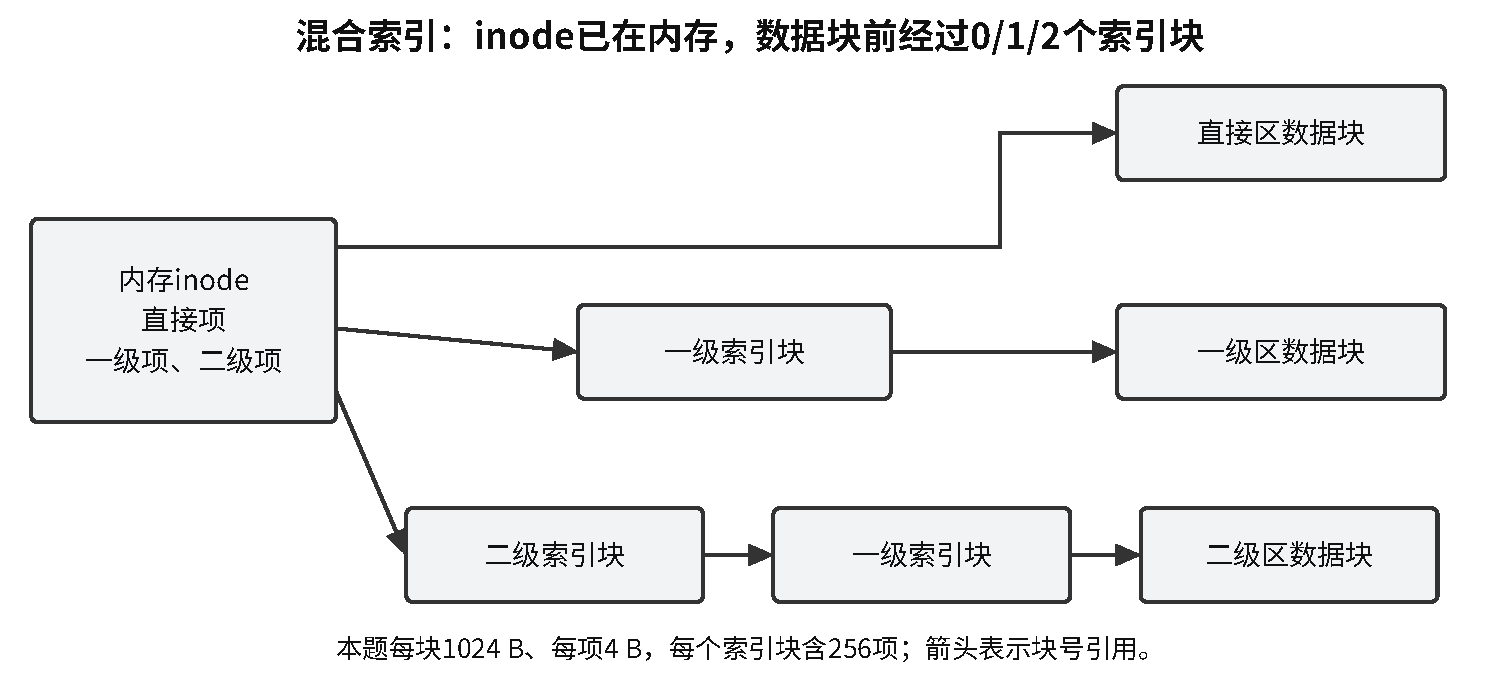
\includegraphics[width=\linewidth,height=125mm,keepaspectratio]{figures/OS_file_index.pdf}
\captionof{figure}{直接、一级、二级路径经过的索引块数不同；图中只画少量代表项}\label{os-fig-index}
\end{minipage}\par\medskip

\end{example}

\textbf{解析。} 一个索引块能存 \(1024/4=256\) 项。直接索引覆盖前 10 KB；一级间接再覆盖 256 KB；二级间接再覆盖 \(256^2\) KB。

1234 小于 \(10\times1024\)，属于直接区。inode 已在内存，可直接取目标块号，只读 1 个数据块。307400 大于 \((10+256)\times1024=272384\)，进入二级区；需读二级索引块、对应的一级索引块和数据块，共 3 次，答案为 \textbf{B}。

还可定位到项：\(307400=300\times1024+200\)，逻辑块号 300；减去前面的 \(10+256=266\) 块，二级区内偏移 34 块，即先取二级索引的第 0 项，再取其所指索引块的第 34 项。块内偏移 200 不影响要经过的索引层数。

本题结构能表示的数据长度为 \((10+256+256^2)\times1024\) B，即 64 MB + 266 KB；其中不把索引块计为文件用户数据长度。若索引块已经缓存，访盘次数会减少；若 inode 尚不在内存，还应计入取得它的相应访问。题目说``索引节点已在内存''，不能再加一次 inode 读盘。

\subsection{例 4-4　链接文件修改一条记录，要把读和写都计入}\label{OS04-ex6-4}

\begin{example}[配套例题]

〖4.2-025〗 一个记录文件采用隐式链接分配，定长逻辑记录为 100 B，采用记录成组分解，盘块为 512 B。目录项已读入内存，对第 22 个逻辑记录完成修改，共启动磁盘多少次？

A. 3　　B. 4　　C. 5　　D. 6

\end{example}

\textbf{解析。} 按原题记录不跨块、每块容纳 5 条记录的模型，第 1---5 条在第 1 块，依次类推，第 22 条位于第 5 块。隐式链要从第 1 块沿后继指针读到第 5 块，共读 5 次，再把修改后的第 5 块写回 1 次，总计 6 次，答案为 \textbf{D}。目录已在内存只免去目录读取，不能免去沿链的数据块读取。

盘块中的链接指针若占用部分字节，本题只要每块剩余空间仍足够容纳 5 条 100 B 记录，结论不变；若允许跨块记录、索引已缓存或采用 FAT，则必须重画访问路径。不要把``修改第 22 条''理解成写 22 次，也不要漏掉最后的回写。

\subsection{FAT与索引表的具体块号轨迹}\label{OS04-fat-example}

课件的FAT模型中，文件aaa从块2开始，后继关系为\(2\to5\to0\to1\to-1\)；文件bbb从块4开始，为\(4\to23\to3\to-1\)。-1表示链尾。aaa的第0、1、2、3号逻辑块分别映射到2、5、0、1号物理块。若FAT已驻留内存，定位第3号逻辑块需要查询内存中的三个链接，但只需为最终数据块发起一次读盘。

同一课件的索引分配例为：aaa的索引块号7，索引项依次保存2、5、13、9，因而逻辑块2直接查第2项得到物理块13。索引块7是元数据块，不是文件的第0号用户数据块。FAT按受管卷组织表项，而块索引通常按文件分别组织。

\subsection{索引块装不下时：链接、多层和混合}\label{OS04-index-extensions}

一个索引块不够时，可以将多个索引块\textbf{链接}：目录记录首个索引块，查后面的索引块还要读取前面的索引块来获得链接。它节省单块容量限制，但不再具备直接到任意索引块的能力。

\textbf{多层索引}让顶层索引指向下层索引块。每块1024 B、地址4 B，则扇出为256；两层索引覆盖\(256^2\)个数据块，即64 MiB。顶层尚未缓存时，读取用户数据要访问顶层、下一层和数据块，共3次。小文件仍会承担固定层级开销。

课件的\textbf{混合索引}含8个直接地址、一个一级间接地址和一个二级间接地址，覆盖

\[(8+256+256^2)\times1\text{ KiB}=65800\text{ KiB}.\]

在顶级控制信息尚未读入内存的题设下，逻辑块0～7、8～263、264～65799分别经过直接、一级间接和二级间接路径，总读盘数为2、3、4；顶级信息已缓存则各减1。该例的8个直接地址与前例10个直接地址是两套数据，计算时各自使用其前提。

\section{目录和路径解析：逐层找到名字}\label{OS04-6-6}

单级目录把所有文件名放在一张表，简单但命名冲突多；两级目录按用户分开，缓解重名但共享和多层分类受限；树形目录让目录内再有子目录，便于按层次组织。绝对路径从根开始，相对路径从当前工作目录开始；\texttt{.\allowbreak{}} 表示当前目录，\texttt{.\allowbreak{}.\allowbreak{}} 表示父目录，二者的解析都受权限与挂载规则约束。

访问 \texttt{/\allowbreak{}home/\allowbreak{}u/\allowbreak{}a.\allowbreak{}txt} 并不是在一张全局名字表里直接跳到数据。典型 inode 模型先从根目录查 \texttt{home}，取得其 inode，再查 \texttt{u}，最后在该目录中查 \texttt{a.\allowbreak{}txt} 并取得文件 inode。各层目录、inode、数据是否缓存，决定实际 I/O 数；路径分量的数量本身不是总访盘次数。

采用``名字与 inode 分离''可以使目录项更小，一块容纳更多名字，从而减少线性查找的目录块数。以王道书 §4.2 的目录模型为例，3200 项、每项 16 B、每块 1024 B，需要 50 个目录块。若目标等概率落在任意一项，且逐块线性查找，各块恰有相同数量目录项，则平均读取 \((1+50)/2=25.5\) 个目录块；随后再读 1 个 inode 块，总期望 26.5 次。用 \(50/2+1=26\) 是``大量目录块''的近似，不能当作相同概率模型下的精确值。

若目录使用哈希或树索引，查找次数应按相应结构计算；若预先只读入目录的一部分，也不能把剩余查找都视为零成本。当前工作目录使常用路径可以省去重复解析共同前缀，但不取消权限检查。

\subsection{课件示例：绝对路径与当前目录}\label{OS04-course-directory}

课件的根目录含\texttt{qianlong}、\texttt{照片}和\texttt{对账单4}；\texttt{qianlong}与\texttt{照片}目录下分别有名为\texttt{demo}的文件，它们属于不同目录，可以同名。\texttt{照片}下的\texttt{2015-08}目录中有\texttt{自拍.\allowbreak{}jpg}和\texttt{自拍2.\allowbreak{}png}。

\begin{wideblock}

\par\medskip\noindent\begin{minipage}{\linewidth}
\centering
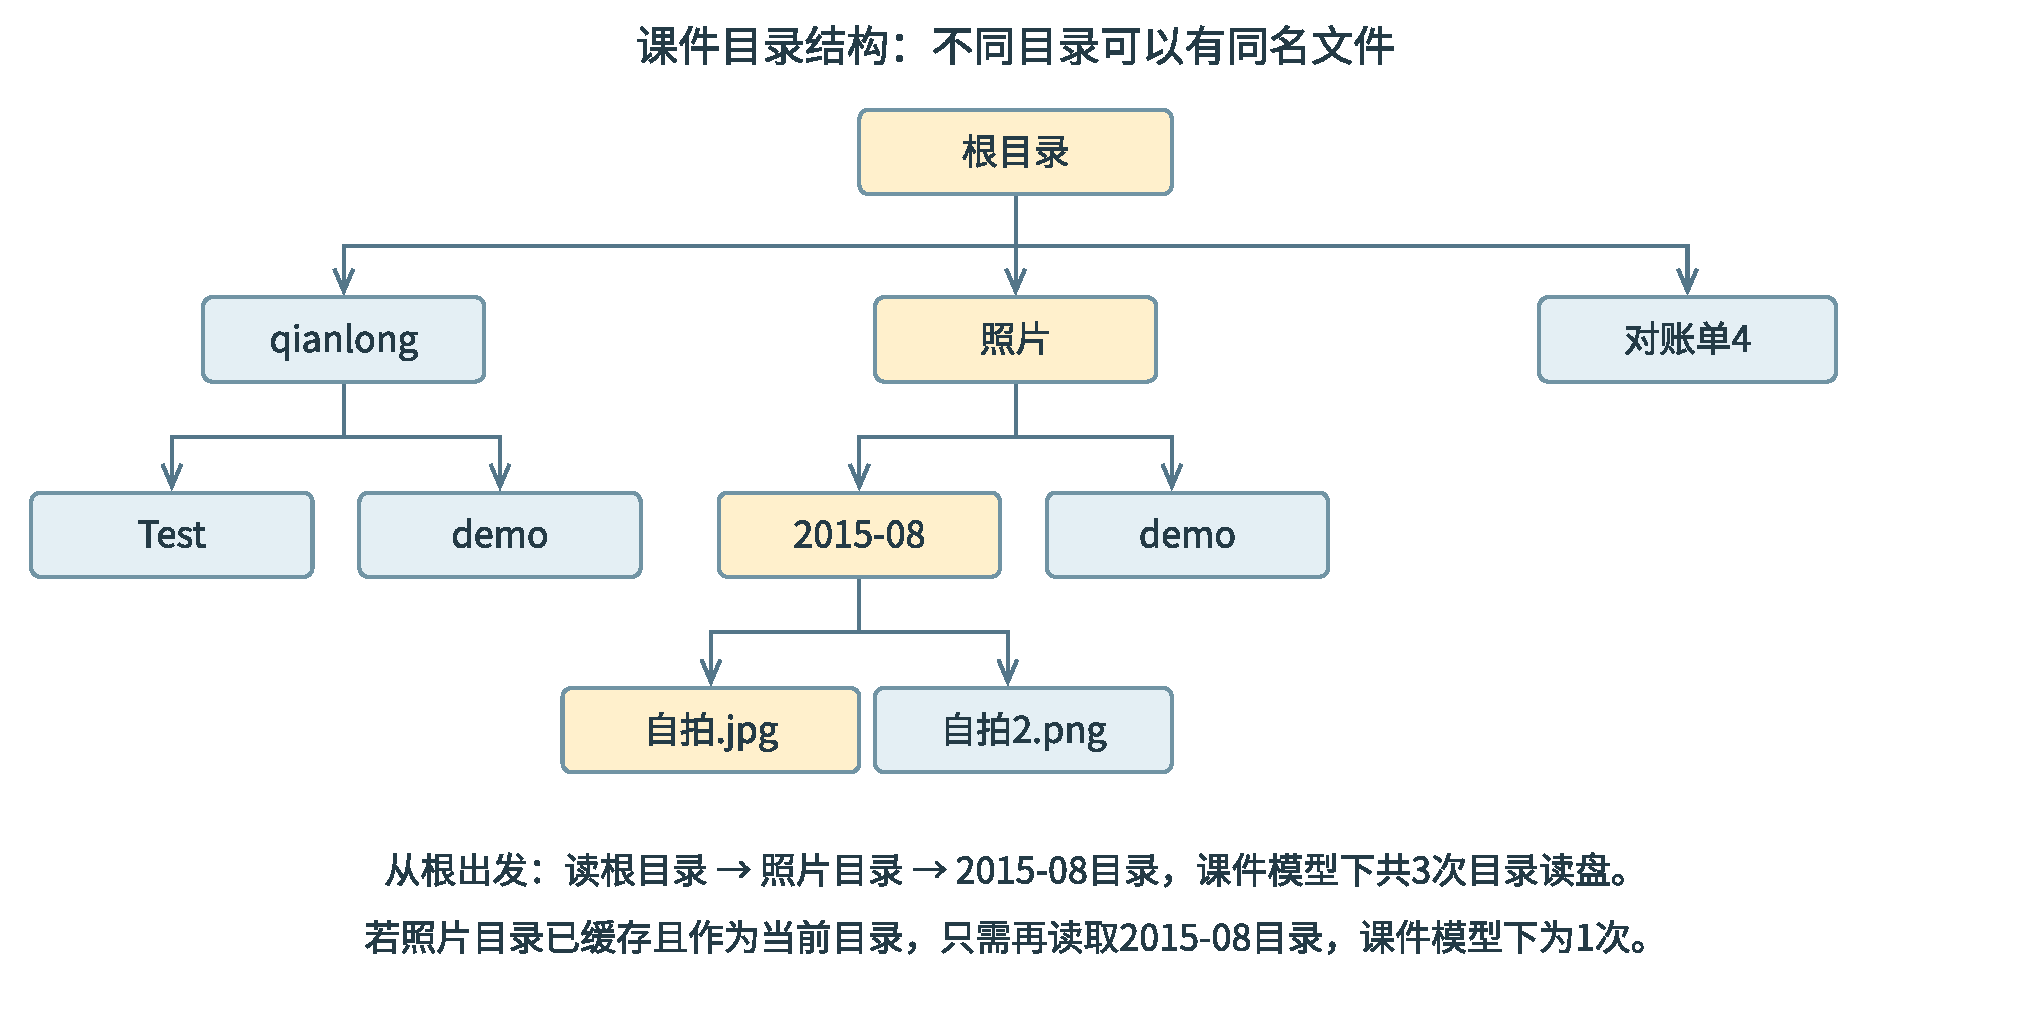
\includegraphics[width=\linewidth,height=125mm,keepaspectratio]{figures/OS_directory_course.pdf}
\captionof{figure}{根目录、qianlong与照片目录、2015-08目录以及文件的父子关系}\label{os-fig-directory-course}
\end{minipage}\par\medskip

\end{wideblock}

\texttt{自拍.\allowbreak{}jpg}的绝对路径为\texttt{/\allowbreak{}照片/\allowbreak{}2015-08/\allowbreak{}自拍.\allowbreak{}jpg}。在课件给定的简化模型里，若根目录、照片目录和2015-08目录的内容初始均不在内存，且每读取一张目录表恰需一次磁盘I/O，则从根开始依次读入三张目录表，需要3次目录读盘；这里统计到找到目录项为止，文件内容或其他未缓存元数据的读取须依题设另计。

若已打开``照片''目录且其目录表驻留内存，把它设为当前目录后，可用相对路径\texttt{.\allowbreak{}/\allowbreak{}2015-08/\allowbreak{}自拍.\allowbreak{}jpg}。查找\texttt{2015-08}时无需重新读取根目录和照片目录，在同一简化模型下只需再读入2015-08目录，故为1次目录读盘。当前目录和缓存是否存在是这个数值成立的前提。

\subsection{无环图目录与目录项瘦身的收益}\label{OS04-directory-dag}

树形目录中的每个非根节点只有一个父目录。无环图目录允许多个父目录引用同一文件，或在受控模型中共享子目录，让用户使用不同名字访问共同对象。为避免形成难以回收的目录环，实际系统通常限制任意硬链接目录；允许什么链接由文件系统政策决定。

共享计数统计指向该对象的目录关联。删除一个名字只取消一条边；仍有其他名字时保留共同内容。共享与复制也不同：共享者修改共同对象，其他名字随后仍访问该对象；复制得到的文件则拥有各自数据和元数据。

将大FCB中的文件名与其余属性分离，可提高每块目录的容纳量。课件数据为640个目录项、原FCB64 B、块长1024 B：原目录每块16项，共40块；改成文件名14 B加索引节点指针2 B后，每块64项，共10块。按成功位置均匀的逐块查找，精确平均目录读盘数分别为\((40+1)/2=20.5\)与\((10+1)/2=5.5\)；课件用``一半''近似为20与5。找到名字以后，再按题给缓存状态计入读取inode的成本。

这种改进让目录查询更紧凑，不是消除了文件属性，也不是所有文件属性都应直接放在一个小目录项里。

\section{硬链接、软链接与什么时候回收文件}\label{OS04-6-7}

\textbf{硬链接}是另一个目录项直接指向同一文件 inode；多个名字地位相同，不存在``原名字一删，另一个就失效''的必然关系。增加一个硬链接通常增加 inode 的硬链接计数，删除一个名字减少计数；只有计数归零，并且不再有有效使用引用等其他条件，才能回收数据和 inode。硬链接通常不能跨文件系统，因为 inode 编号必须在本文件系统解释；通常也限制用户为目录建立硬链接，以避免目录环等管理问题。

\textbf{软链接或符号链接}是一个特殊文件，内容保存目标路径。访问软链接时，系统再解析这个路径；目标被删或移走后，软链接本身仍可存在，只是成为悬空链接。它可以跨文件系统，也可指向目录；相对目标路径的解释与链接所在位置有关，不能一概按调用者当前工作目录处理。

\par\medskip\noindent\begin{minipage}{\linewidth}
\centering
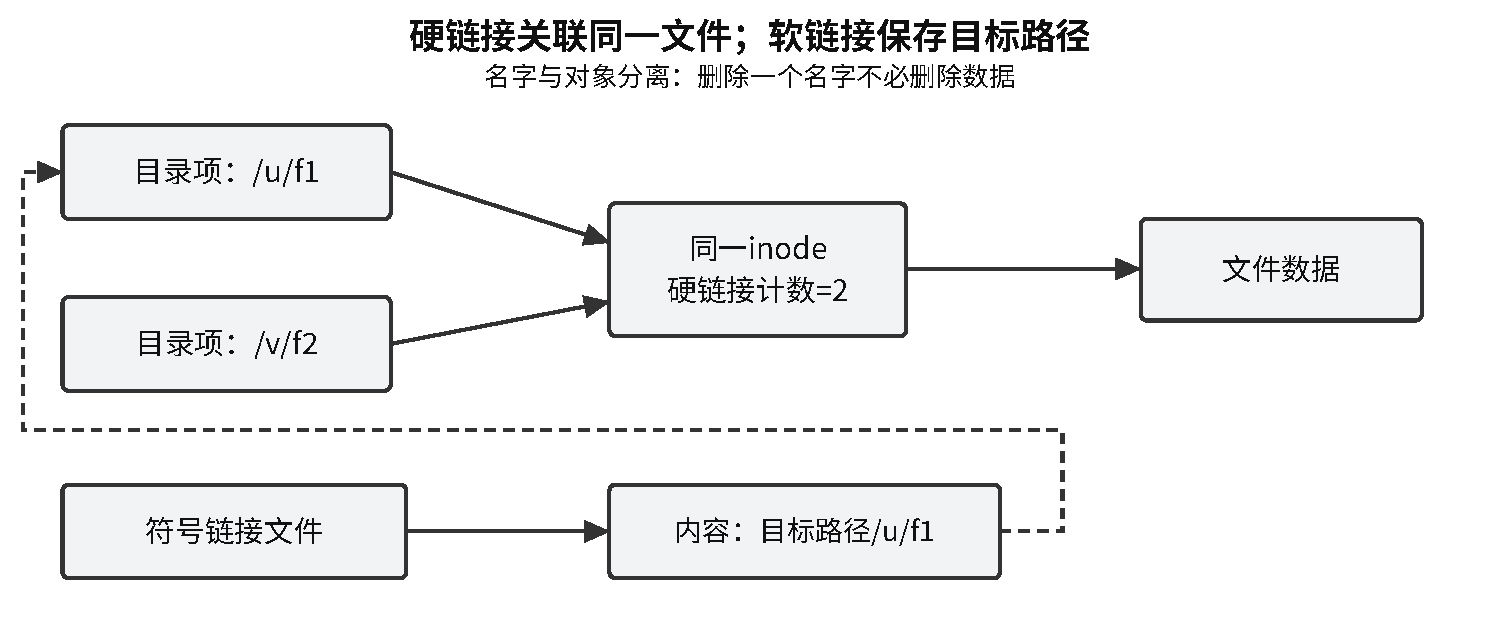
\includegraphics[width=\linewidth,height=125mm,keepaspectratio]{figures/OS_file_links.pdf}
\captionof{figure}{两个硬链接指向同一 inode；软链接保存路径，经过名称解析再找到目标}\label{os-fig-links}
\end{minipage}\par\medskip

\subsection{课件示例：硬链接计数与符号链接的路径}\label{OS04-course-link-path}

课件中，User1 的目录项 \texttt{aaa} 和 User2 的目录项 \texttt{bbb} 都指向 inode 1，硬链接计数为 2；User3 的目录项 \texttt{ccc} 指向另一个 inode 2，其文件内容为目标路径 \texttt{C:\allowbreak{}/\allowbreak{}User1/\allowbreak{}aaa}。访问 \texttt{ccc} 时，系统先读取这个符号链接保存的路径，再按该路径查找目标。

\begin{wideblock}

\par\medskip\noindent\begin{minipage}{\linewidth}
\centering
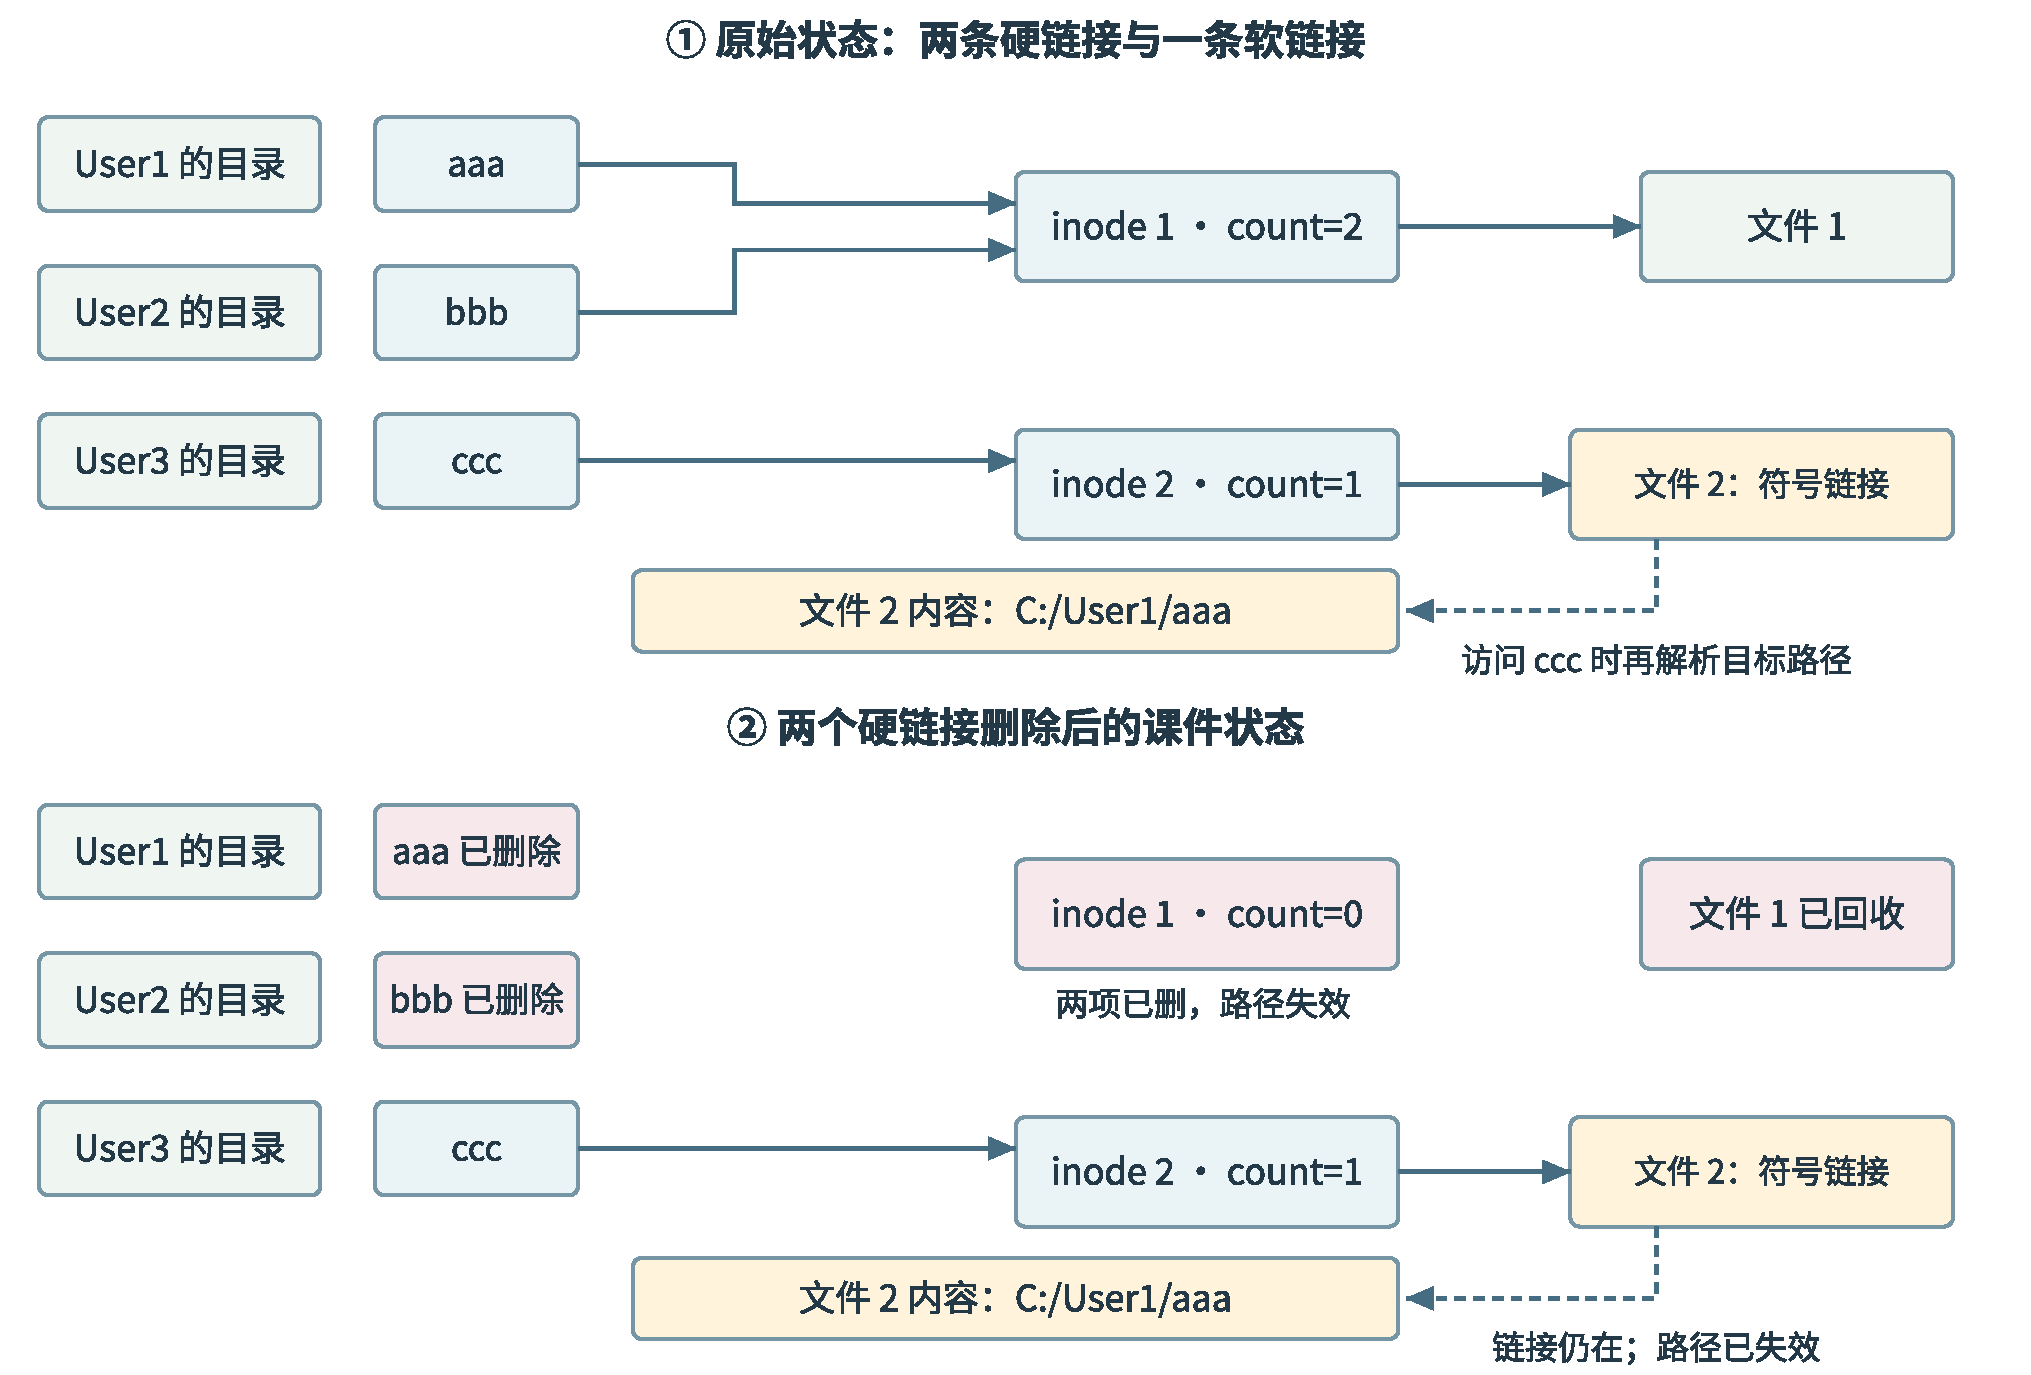
\includegraphics[width=\linewidth,height=125mm,keepaspectratio]{figures/OS_links_course.pdf}
\captionof{figure}{课件中的两条硬链接、符号链接及删除后路径失效状态}\label{os-fig-links-course}
\end{minipage}\par\medskip

\end{wideblock}

若两个硬链接对应目录项均被删除，inode 1 的硬链接计数为 0。在课件假定不存在其他有效打开引用的情形下，文件 1 可以回收。符号链接文件 2 与 \texttt{ccc} 目录项仍存在，但其保存的路径已找不到 \texttt{aaa}，因此是悬空链接；若文件仍有打开引用，实际回收还须等待相应引用释放。只删除 \texttt{aaa} 时，即使 \texttt{bbb} 仍能访问文件，\texttt{ccc} 保存的特定路径也已失效。

\subsection{例 4-5　同一 inode 不要求同一读写位置}\label{OS04-ex6-5}

\begin{example}[配套例题]

【配套例题】 若文件 f1 的硬链接为 f2，两个进程分别打开 f1、f2，获得文件描述符 fd1、fd2，则正确的是（　）。

\ensuremath{\mathrm{I}}. f1 和 f2 的读写指针位置保持相同

\ensuremath{\mathrm{II}}. f1 和 f2 共享同一个内存索引节点

\ensuremath{\mathrm{III}}. fd1 和 fd2 分别指向各自的用户打开文件表中的一项

A. 仅\ensuremath{\mathrm{III}}　　B. 仅\ensuremath{\mathrm{II}}、\ensuremath{\mathrm{III}}　　C. 仅\ensuremath{\mathrm{I}}、\ensuremath{\mathrm{II}}　　D. \ensuremath{\mathrm{I}}、\ensuremath{\mathrm{II}}、\ensuremath{\mathrm{III}}

\end{example}

\textbf{解析。} f1、f2 是同一文件的两个名字，两次打开最终引用同一个 inode，\ensuremath{\mathrm{II}}正确。两进程分别打开，读写位置可以独立，\ensuremath{\mathrm{I}}错误。每个文件描述符在相应进程的描述符表中解释，分别关联各自的打开表项，\ensuremath{\mathrm{III}}正确。答案为 \textbf{B}。这与共享同一个打开实例的继承或复制描述符情形不同。

\section{文件系统分层：从用户请求到块设备}\label{OS04-fs-layers}

文件系统把一个名称层的请求分解为查目录、验证权限、定位记录、转换块地址和操作设备等职责。课件采用下表的分层方法；教材还可把相近职责合并为逻辑文件系统、文件组织模块、基本文件系统和I/O控制，层名有所不同，但应能将每项职责放到正确位置。

\par\medskip\noindent\begin{minipage}{\linewidth}\fontsize{9.3}{12}\selectfont\begin{tabularx}{\linewidth}{@{}YY@{}}
\toprule\noalign{}
\begin{minipage}[b]{\linewidth}\raggedright
层次／模块
\end{minipage} & \begin{minipage}[b]{\linewidth}\raggedright
主要职责
\end{minipage} \\
\midrule\noalign{}


用户接口 & 接收open、read、write、close等系统调用请求 \\
文件目录系统 & 按路径查找FCB或inode，管理目录和打开信息 \\
存取控制模块 & 检查主体是否拥有相应访问权限 \\
逻辑文件系统与文件信息缓冲区 & 将记录号等逻辑使用位置转换为文件逻辑地址 \\
物理文件系统 & 将文件逻辑地址转换为外存物理位置 \\
辅助分配模块 & 分配和回收文件存储空间 \\
设备管理模块 & I/O缓冲、设备调度、启动及完成处理等设备服务 \\
\bottomrule\end{tabularx}
\end{minipage}\par\medskip

\par\medskip\noindent\begin{minipage}{\linewidth}
\centering
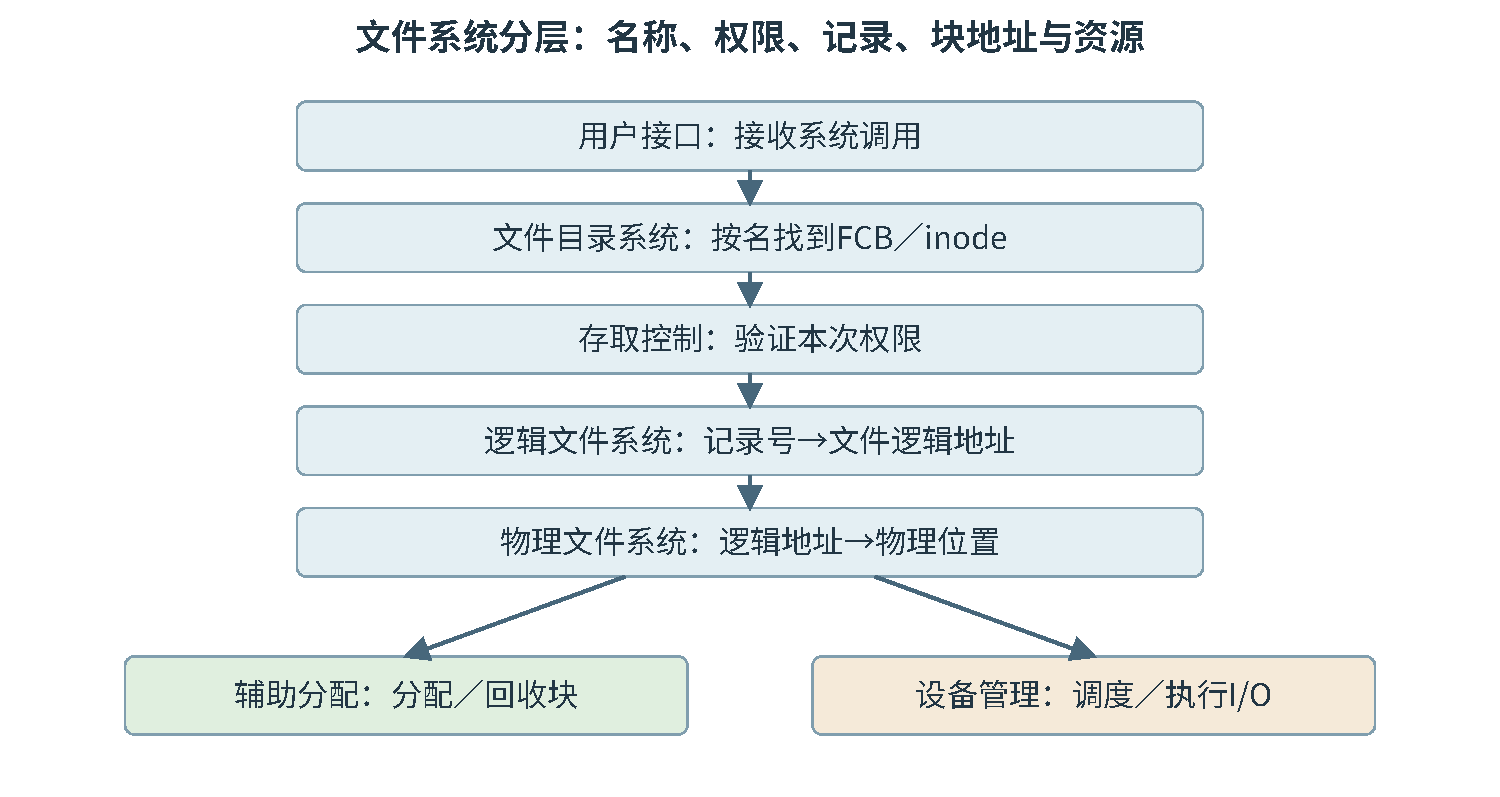
\includegraphics[width=\linewidth,height=125mm,keepaspectratio]{figures/OS_file_layers.pdf}
\captionof{figure}{删除文件末尾记录时，各层完成名称、权限、地址和资源更新}\label{os-fig-file-layers}
\end{minipage}\par\medskip

例如删除\texttt{/\allowbreak{}工作目录/\allowbreak{}学生信息.\allowbreak{}xlsx}末尾100条记录：接口接收请求，目录系统找到文件，存取控制验证权限，逻辑层确定被删除记录的逻辑范围，物理层定位相应块，设备管理执行必要更新，辅助分配回收不再需要的空间。若末块仍含保留记录，则只调整文件长度等信息，不能把整块中有效数据一并释放。

\section{文件系统的磁盘结构与内存结构}\label{OS04-6-8}

磁盘上的引导控制信息用于启动；卷控制块或超级块记录块大小、卷规模、空闲管理等总体信息；目录和 inode 区描述对象与名字；数据区保存内容。具体文件系统可采用其他布局，题目若给不同结构，应以其字段为准。超级块并不保存每个文件的索引信息。

\par\medskip\noindent\begin{minipage}{\linewidth}
\centering
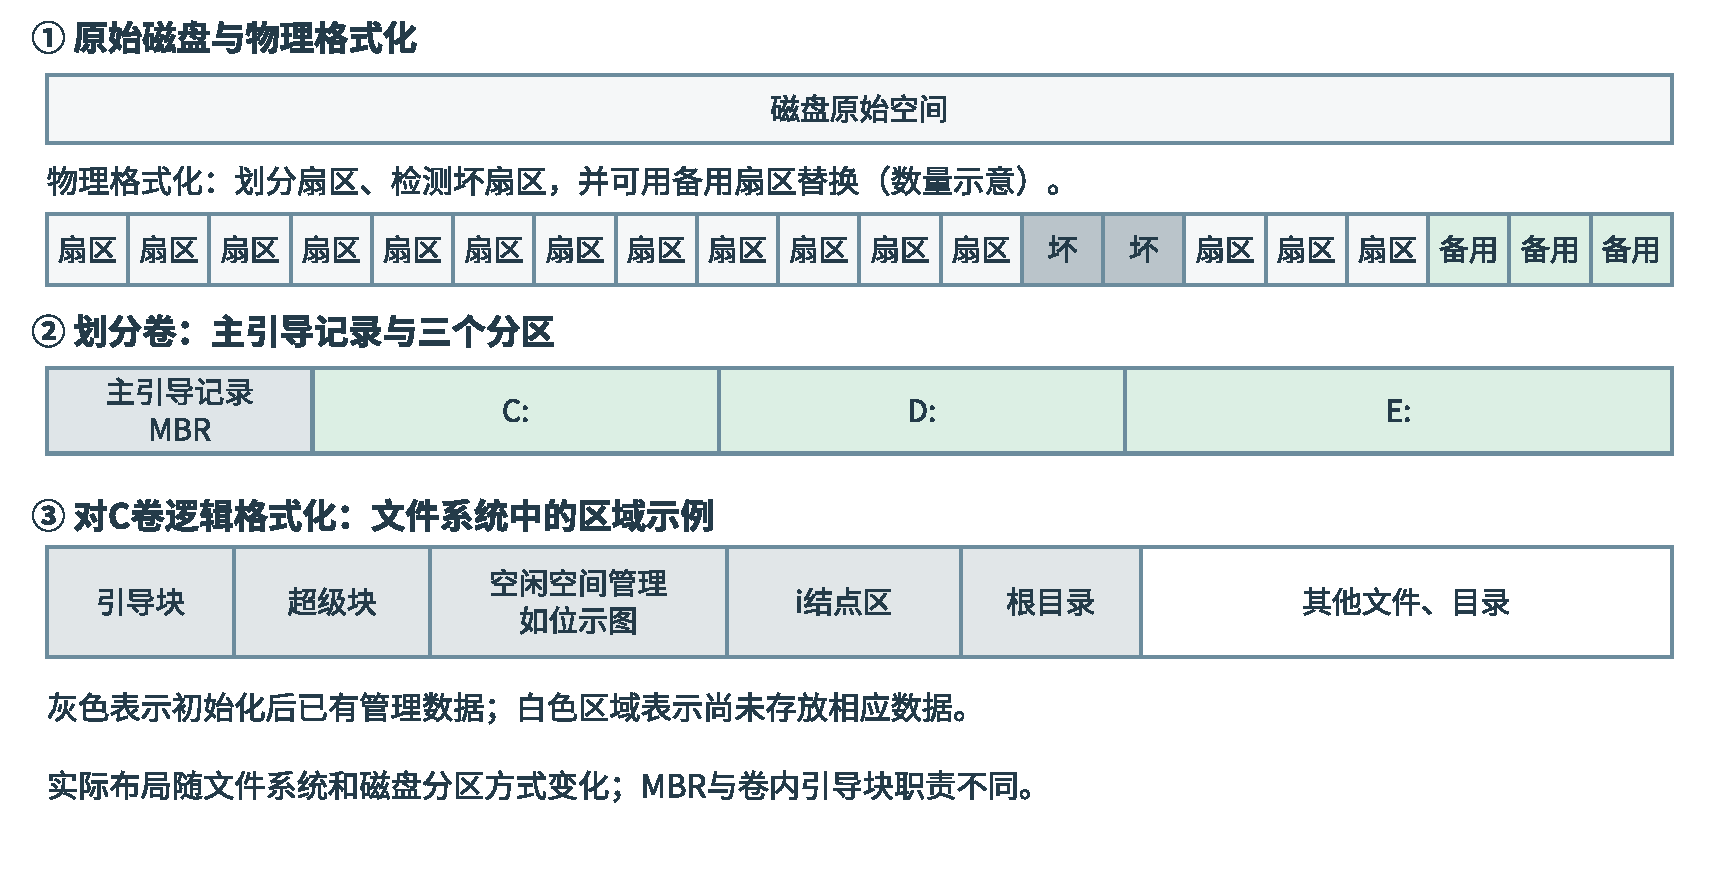
\includegraphics[width=\linewidth,height=125mm,keepaspectratio]{figures/OS_filesystem_layout.pdf}
\captionof{figure}{物理格式化划分扇区并处理坏扇区，分区后对C卷逻辑格式化得到卷内管理区}\label{os-fig-filesystem-layout}
\end{minipage}\par\medskip

在课件的MBR示例中，磁盘包含主引导记录和C、D、E三个分区。对C卷逻辑格式化后，卷内依次示出引导块、超级块、空闲空间管理信息、i结点区、根目录和其他文件／目录区域；图示灰色部分已有初始化数据。MBR属于整个磁盘的引导与分区管理信息，卷内引导块属于该卷的引导信息；二者所在位置和职责不同。上述排列是该教学模型，不代表所有文件系统都按相同顺序放置。

挂载后，内存中维护已挂载文件系统信息、目录缓存、inode 缓存、系统打开对象以及进程描述符表等。缓存加快访问，但修改与写回必须遵守规定的次序和时机。一次文件扩展可能同时修改数据块、空闲位图、inode 大小和块地址；若只写了一部分就断电，会出现泄漏或结构不一致。

一致性检查可以扫描目录、inode 与块使用关系，找出不一致；日志机制先记录需要完成的更新，再按规则提交和重放，减少崩溃后恢复工作。日志不表示任意用户数据都自动获得完整事务语义，其保证取决于记录元数据还是数据、提交和写回的具体规则。这里只解释多结构更新之间的因果，不展开某种文件系统的实现细节。

\section{空闲空间：位图、空闲链和成组链接}\label{OS04-6-9}

\textbf{空闲表}记录连续空闲区的起点与长度，适合按区段管理；\textbf{空闲链}把空闲块或空闲区串起来；\textbf{位图}为每个受管块保留一位，值表示空闲或占用，具体 0、1 意义由题目规定；\textbf{成组链接}把若干空闲块号存成一组，用组内的连接信息指向后续组，并在内存保留当前组的块号栈。

位图大小主要由受管总块数决定，不随当前空闲块数改变；空闲表、空闲链所需内容则与当前空闲分布相关。成组链接靠少量的组间连接把大量空闲块号组织起来，并不是把所有文件的数据链混在一起。

\subsection{空闲表、盘块链和盘区链怎样分配与回收}\label{OS04-free-methods}

空闲表的每项为``起始空闲块号、连续块数''。申请连续的\(K\)块时，可以用首次适应、最佳适应或最坏适应选区；分配后缩小或删除表项。回收时依地址检查前邻、后邻、两侧相邻或两侧均不相邻四种情况，分别扩展、三段合并或新建表项，与内存动态分区的物理邻接判断相同。

课件示例中，空闲区依地址排列，首次适应为新文件分配3块：起始于0的2块和起始于5的1块都不足，选中10～14并分配10～12，留下13～14。此时另有空闲区18～20；回收15～17后，按物理地址合并13～14、15～17、18～20，得到起始块13、长度8的空闲区。

空闲\textbf{盘块链}把每个空闲块链接起来，内核保存链头等信息，申请\(K\)块就依次摘取\(K\)个节点，回收块再挂回链。它适合离散分配，但申请多个块可能要多次追链。空闲\textbf{盘区链}每节点代表一段连续空闲区，首块保存长度和后继盘区信息，一次可分出多个块；回收时仍要检查相邻盘区合并。

位图适用于连续或离散分配。按课件的0基模型，字长\(n\)位、字号\(i\)、位号\(j\)对应盘块号

\[b=ni+j,\qquad i=\lfloor b/n\rfloor,\qquad j=b\bmod n.\]

\(n=16\)时，\((i,j)=(1,10)\)对应块26；块31对应\((1,15)\)。若题目按教材另一模型让块号、字号、位号都从1开始，则应为

\[b=n(i-1)+j,\quad i=\lfloor(b-1)/n\rfloor+1,\quad j=(b-1)\bmod n+1.\]

两套定义必须整套使用。分配时找空闲位并改为占用，回收时做相反更新；0代表空闲还是占用先读题设。

\subsection{成组链接：组满、组空时怎样转移}\label{OS04-grouped-free}

在课件每组最多100个块号的模型中，内存超级块缓存当前组；该组最后取出的某个空闲块同时存放下一组目录。组内块号不要求连续。

\begin{wideblock}

\par\medskip\noindent\begin{minipage}{\linewidth}
\centering
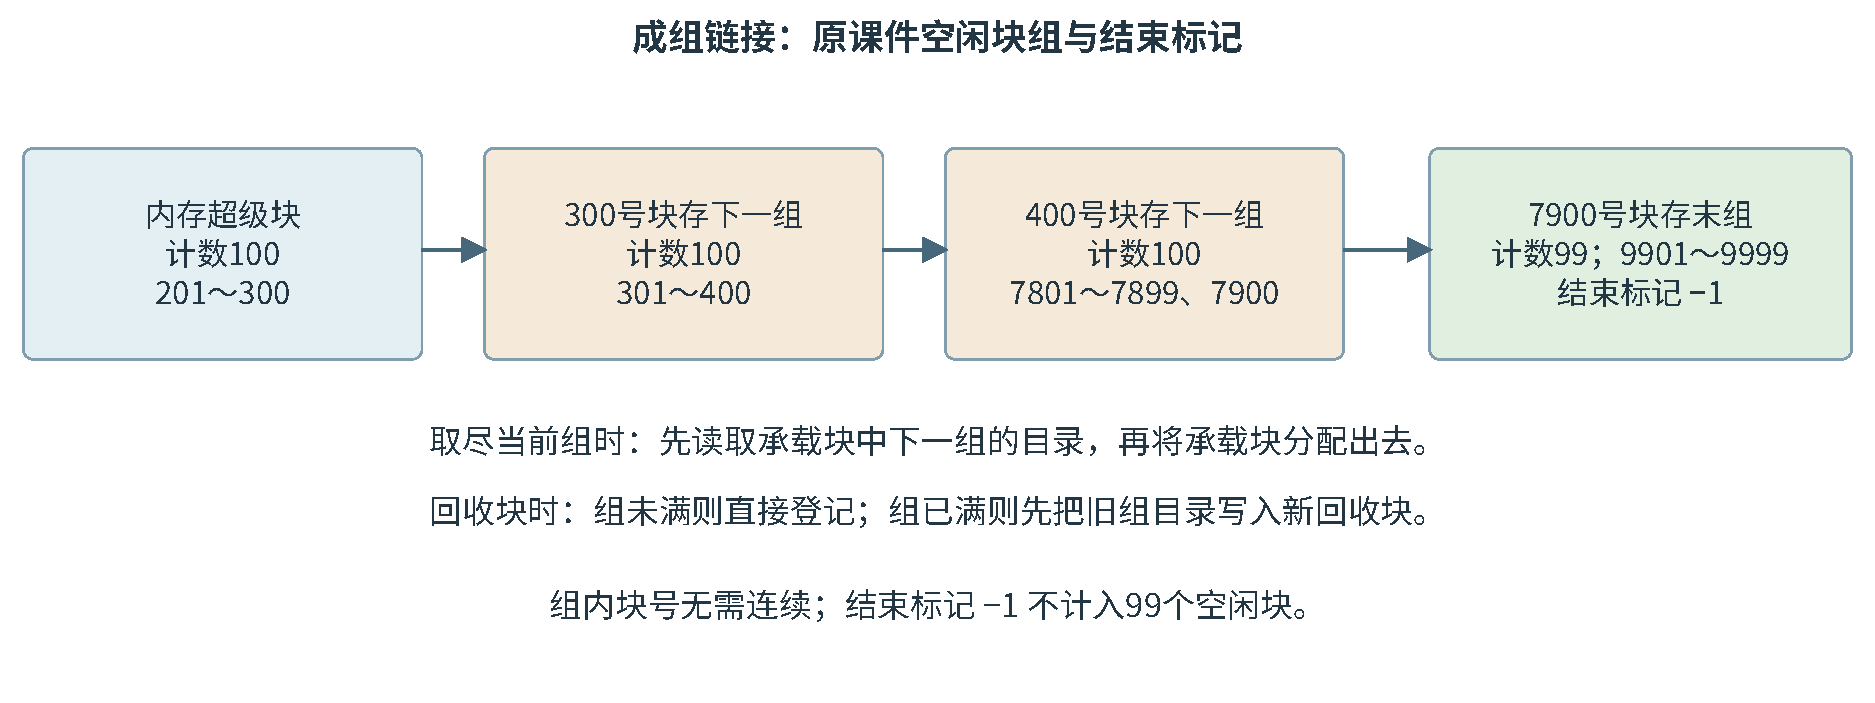
\includegraphics[width=\linewidth,height=125mm,keepaspectratio]{figures/OS_grouped_free.pdf}
\captionof{figure}{当前组用尽时先从承载块装入下一组，再把承载块交付使用}\label{os-fig-grouped-free}
\end{minipage}\par\medskip

\end{wideblock}

假设当前组登记201～300共100个空闲块，300号块内登记下一组301～400。申请1块时可取出201并将计数由100改为99；申请至当前组用尽时，先把300号块中保存的下一组信息读入超级块，再把300也交给申请者。若先覆盖300的内容，下一组入口就会丢失。 课件继续给出：400号块记录的下一组含7801～7899和7900共100个块；7900号块记录末组9901～9999共99个块，连接位置的特殊值 \(-1\) 表示没有后续组，不计入99个空闲块。

回收时，当前组未满则将块号压入并增加计数；当前组已满又回收一个新块\(x\)，先把当前100项组信息写到\(x\)中，再让超级块仅保存\(x\)作为新组入口。以后分配到\(x\)时，就能恢复被保存的那一组。末组以专门的结束标记表示无后续组，不能把标记当成可分配块号。

超级块的内存状态及磁盘状态要按规定同步；位图、空闲表和组目录都属于分配元数据，与文件自己的数据块索引分别管理。

\subsection{例 4-6　先定位位图块，再定位块内字节}\label{OS04-ex6-6}

\begin{example}[配套例题]

【配套例题】 文件系统用位图表示磁盘空间分配，位图存于磁盘 32---127 号块，每块 1024 B，盘块和块内字节都从 0 编号。释放盘块号 409612 时，要修改的位所在盘块号和块内字节序号分别为（　）。

A. 81、1　　B. 81、2　　C. 82、1　　D. 82、2

\end{example}

\textbf{解析。} 每个盘块的位图可表示 \(1024\times8=8192\) 个数据块。\(409612=50\times8192+12\)，故目标位在位图第 50 块，即磁盘块 \(32+50=82\)；余数即块内第 12 位，它位于字节 \(\lfloor12/8\rfloor=1\)，在该字节中的位序号为 4。答案为 \textbf{C}。

位图自身的起始磁盘块号 32，只在``位图内相对块号''算出以后加；不能先把受管盘块号减去 32。修改成 0 还是 1，要看位图的空闲值约定，本题只问位置，不必自行确定。

\section{虚拟文件系统与挂载}\label{OS04-6-10}

\textbf{虚拟文件系统 VFS}为不同具体文件系统提供共同的操作抽象，把打开、查找、读写等请求通过相应操作接口分派给具体实现。统一接口不表示磁盘格式也统一，更不要求所有设备保存相同的 inode 布局。

课件先用未统一接口的教学模型说明差异：P1 要分别使用示意的 \texttt{open(\allowbreak{}a,\allowbreak{}b)\allowbreak{}}、\texttt{fopen(\allowbreak{}x)\allowbreak{}} 和 \texttt{openf(\allowbreak{}p,\allowbreak{}q)\allowbreak{}} 访问 UFS、NTFS 和 FAT，不同接口参数与具体实现相互绑定。这里的函数名用于表达接口差异，不是对这些文件系统现实API的逐一规定。

\begin{wideblock}

\par\medskip\noindent\begin{minipage}{\linewidth}
\centering
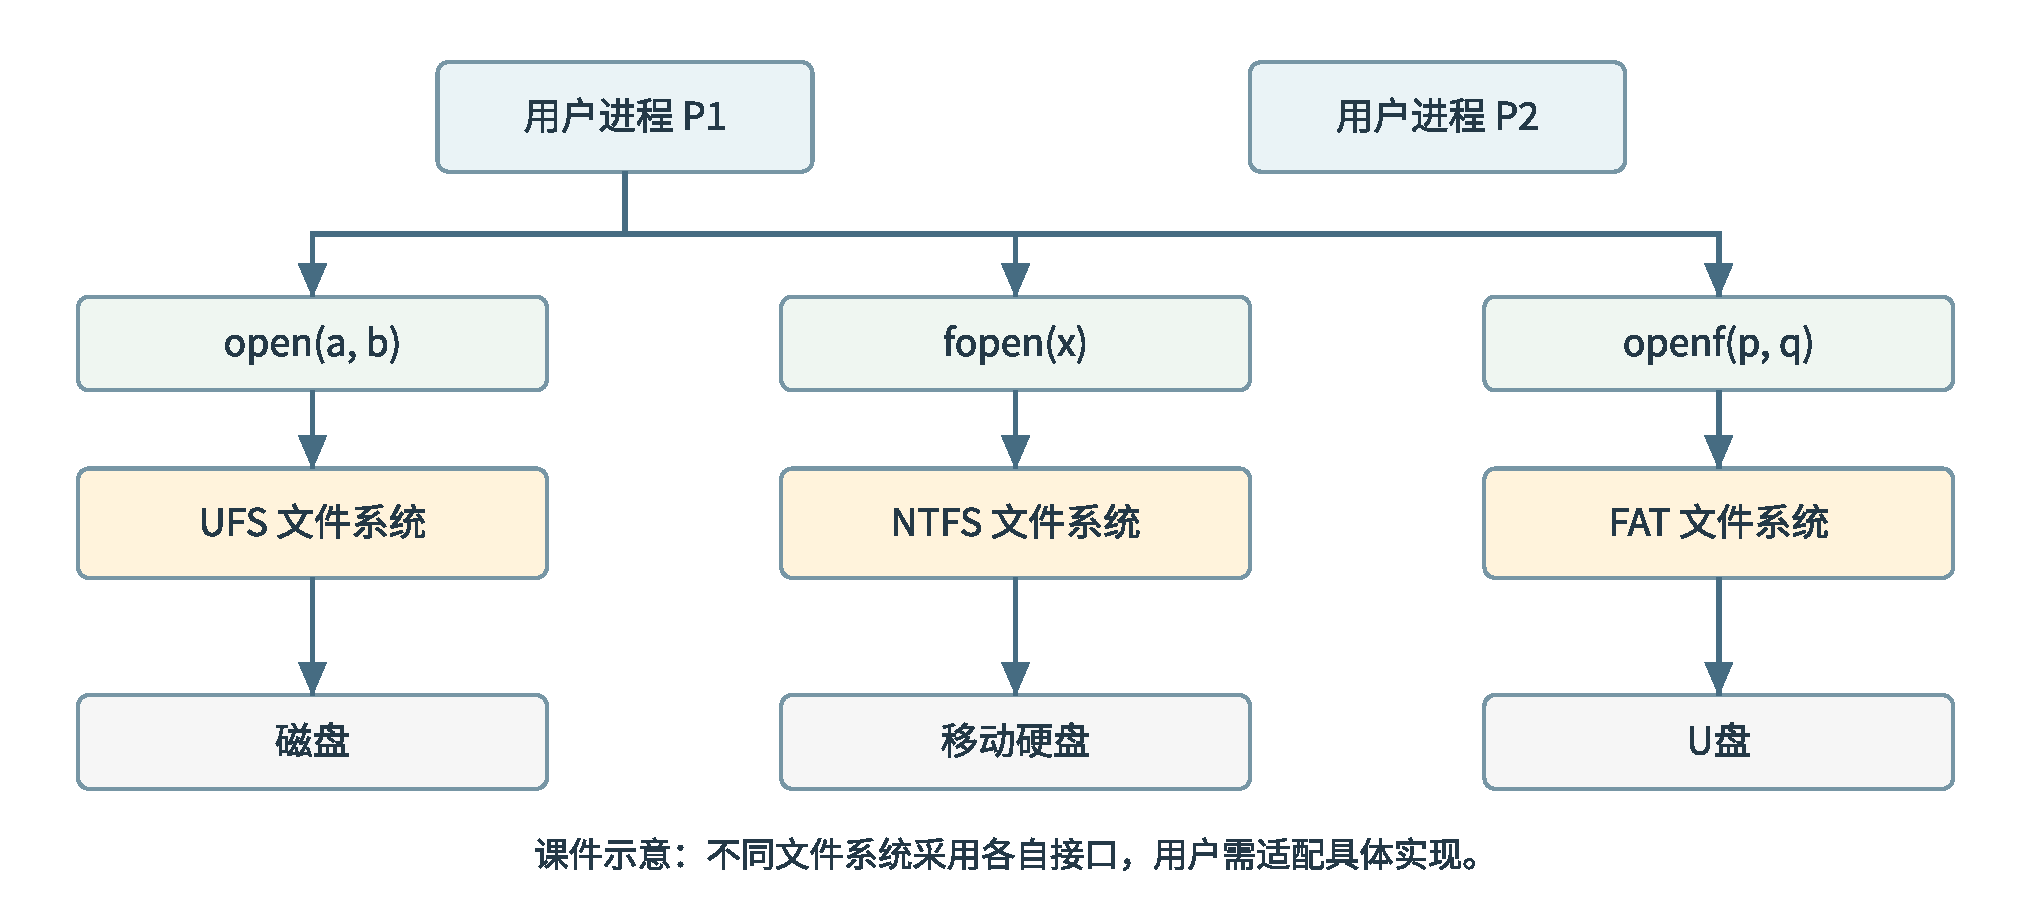
\includegraphics[width=\linewidth,height=125mm,keepaspectratio]{figures/OS_vfs_before_course.pdf}
\captionof{figure}{课件示意：没有统一接口时，P1分别调用三种文件系统的不同接口}\label{os-fig-vfs-before-course}
\end{minipage}\par\medskip

\end{wideblock}

Linux 式抽象常区分超级块对象、inode 对象、目录项对象 dentry 和文件对象：其中超级块对象描述一个已挂载文件系统，inode 描述文件本体，dentry 缓存名字与父目录等关系，file 对象描述一次打开。dentry 与 inode 不是同一个英文术语；目录项对象的名称不能误写成 inode 对象。

\textbf{挂载}把某文件系统的根关联到现有名称空间的一个挂载点，使路径解析到该处时转入新文件系统。挂载点之下原有内容不因此被删除，只是在相应名称解析视图下被新挂载内容遮住。卸载要处理尚在使用的对象和待写回信息，不能只删一个路径字符串就认为设备已经可以安全移除。

\subsection{VFS的统一对象与具体操作入口}\label{OS04-vnode}

课件用\textbf{vnode}表示打开文件时在内存中使用的统一虚拟节点，它保存通用文件信息，并通过操作函数指针转入具体文件系统的open、read、write等实现。vnode是内存抽象，磁盘上的inode格式则由具体文件系统决定；不能要求所有磁盘都直接存放同一种vnode。

\begin{wideblock}

\par\medskip\noindent\begin{minipage}{\linewidth}
\centering
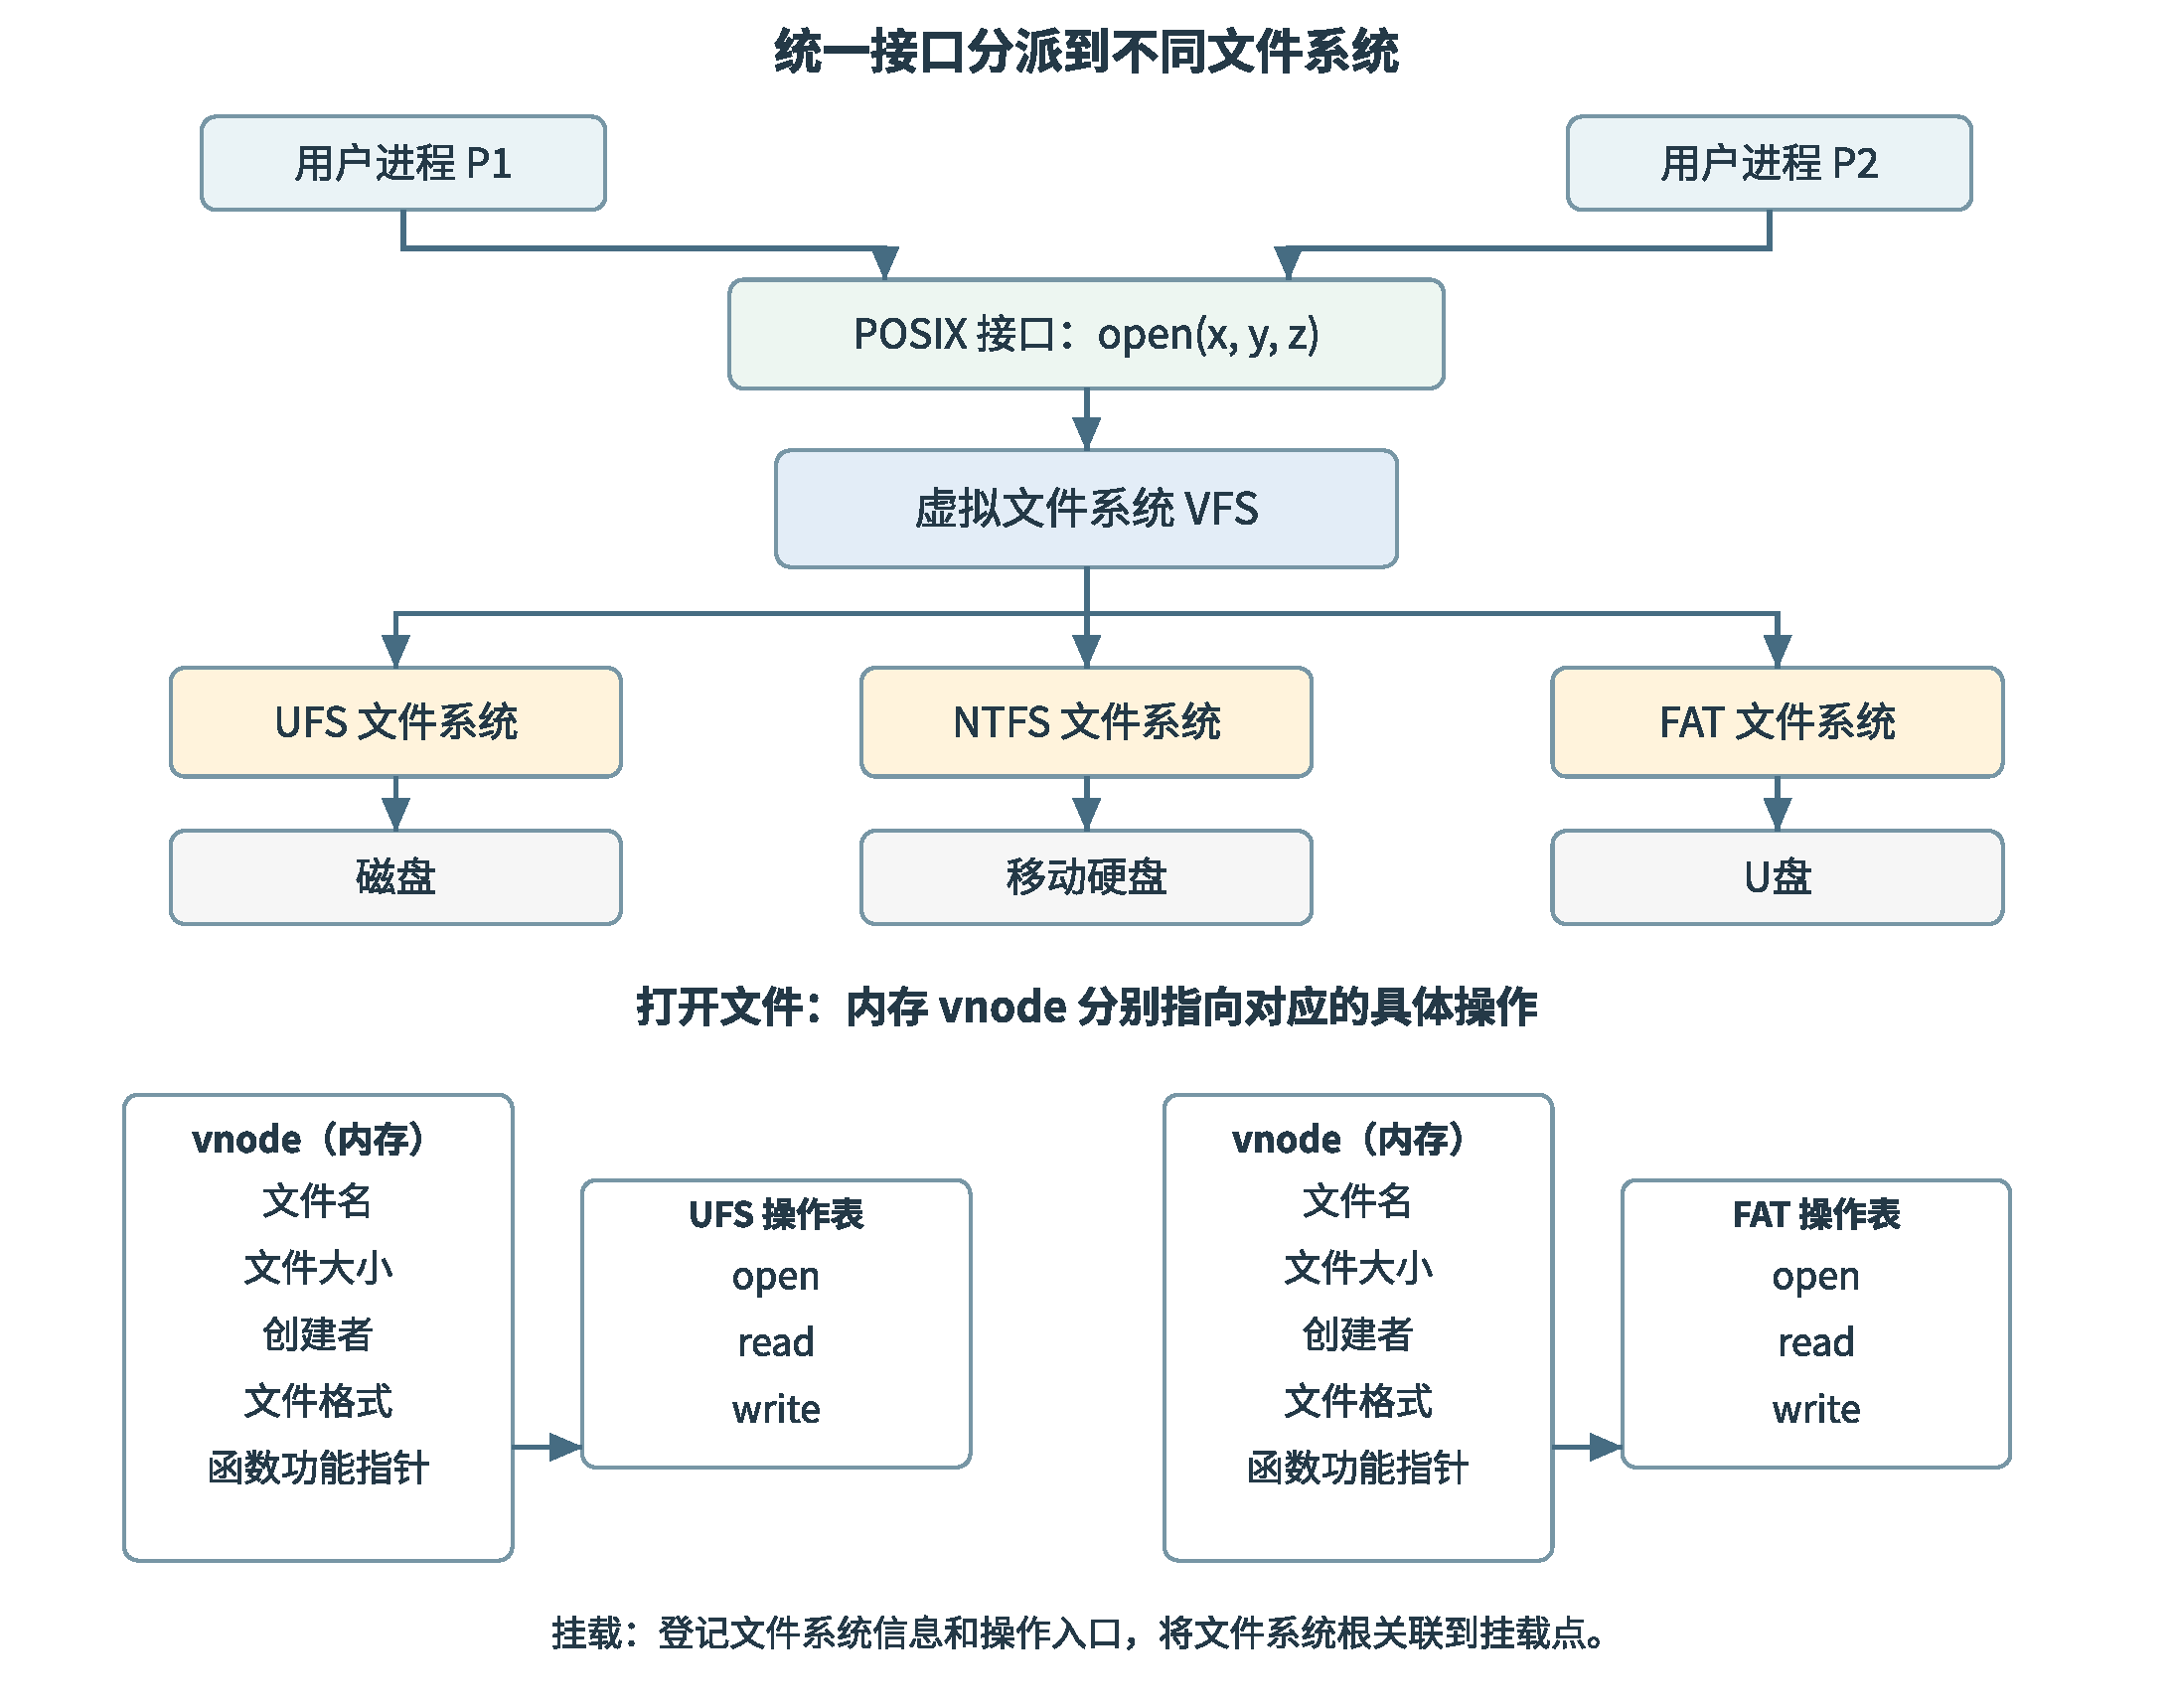
\includegraphics[width=\linewidth,height=125mm,keepaspectratio]{figures/OS_vfs_course.pdf}
\captionof{figure}{课件中的POSIX接口、VFS与UFS、NTFS、FAT分派，以及不同vnode操作表}\label{os-fig-vfs-course}
\end{minipage}\par\medskip

\end{wideblock}

例如图中用户进程通过统一接口请求操作，VFS再根据目标文件所属的具体文件系统转交给UFS、NTFS或FAT。课件示意的vnode记录文件名、大小、创建者、文件格式等通用信息，函数功能指针指向相应具体实现的 \texttt{open}、\texttt{read}、\texttt{write} 等操作。图中的磁盘、移动硬盘和U盘只表示三个具体文件系统实例，介质与文件系统的对应关系由实际格式化和挂载情况决定。

挂载时要在VFS登记文件系统信息，提供所需操作入口，并把其根关联到一个挂载点。随后同样的路径和调用接口可以转入不同底层实现。课件的vnode模型与前述Linux式inode/dentry/file等细分对象，是说明统一抽象的不同组织方法，不能用一张对象表替代另一模型的全部关系。

\section{综合例题：目录、索引与容量共同约束}\label{OS04-6-11}

\subsection{例 4-7　同一索引节点怎样连接目录查找与文件扩展}\label{OS04-ex6-7}

{\tcbset{SNbase/.append style={breakable=false}}\begin{example}[配套例题]

【配套例题】 某文件系统的磁盘块大小为 4 KB，目录项由文件名和索引节点号构成，每个索引节点占 256 字节，其中包含直接地址项 10 个，一级、二级和三级间接地址项各 1 个，每个地址项占 4 字节。该文件系统中子目录 stu 的结构如下图所示，stu 包含子目录 course 和文件 doc，course 子目录包含文件 course1 和 course2。各文件的文件名、索引节点号、占用磁盘块的块号如图中表所示。请回答下列问题。

\par\medskip\noindent\begin{minipage}{\linewidth}
\centering
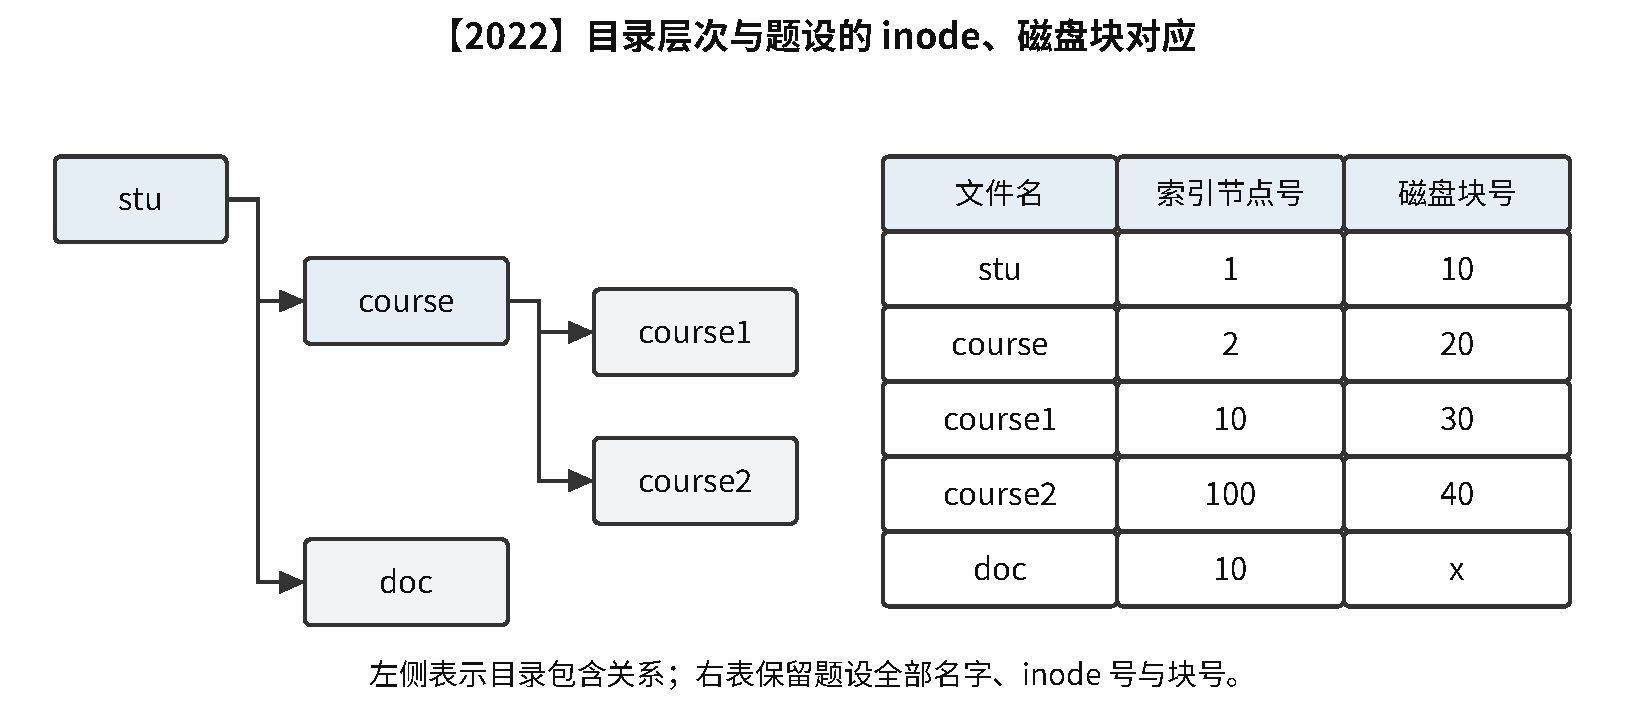
\includegraphics[width=\linewidth,height=125mm,keepaspectratio]{figures/OS_file_directory_2022.pdf}
\captionof{figure}{stu、course 的目录层次，以及各文件的索引节点号和数据块号}\label{os-fig-directory2022}
\end{minipage}\par\medskip

（1）目录文件 stu 中每个目录项的内容是什么？

（2）文件 doc 占用的磁盘块的块号 x 的值是多少？

（3）若目录文件 course 的内容已在内存，则打开文件 course1 并将其读入内存，需要读几个磁盘块？说明理由。

（4）若文件 course2 的大小增长到 6 MB，则为了存取 course2 需要使用该文件索引节点的哪几级间接地址项？说明理由。

\end{example}}

\textbf{解析。} （1）stu 的直接子项只有 course 和 doc。目录项存名字和 inode 号，不存其数据块号，故内容分别为 \texttt{(\allowbreak{}course,\allowbreak{}2)\allowbreak{}}、\texttt{(\allowbreak{}doc,\allowbreak{}10)\allowbreak{}}；course1、course2 的目录项在 course 中，不在 stu 中。图未列出 \texttt{.\allowbreak{}}、\texttt{.\allowbreak{}.\allowbreak{}}，本问按图列出两个给定子项。

（2）doc 和 course1 的索引节点号同为 10，且属于同一文件系统，说明它们是同一个文件对象的两个名字。course1 的数据在 30 号磁盘块，因此 \(x=30\)。不是因为名字相似而共享，也不是把 inode 号 10 直接当作数据块号。

（3）按本问给出的缓存起点，course 的目录项可在内存查到，先取得 course1 的 inode 号 10。随后读入该 inode 所在的磁盘块，从 inode 得到数据块号 30，再读 30 号数据块，共 \textbf{2 个磁盘块}。打开所需的内存表项由系统建立，不另算作磁盘块；256 B 的 inode 放在磁盘块中，读取它仍按块计。题目只说目录内容已在内存，不能顺带认定文件 inode 和数据也已经缓存；若另给这些缓存命中条件，才相应减少次数。

（4）本题按 \(1\text{ MB}=1024\text{ KB}\) 计算，6 MB 文件需要

\[\frac{6\times1024\text{ KB}}{4\text{ KB}}=1536\text{ 个数据块}.\]

每个间接索引块容纳 \(4096/4=1024\) 个地址项。10 个直接项与一级间接项合计覆盖 \(10+1024=1034\) 个数据块，仍少 \(1536-1034=502\) 块；二级间接项可再覆盖 \(1024^2\) 个数据块。因此需用\textbf{一级和二级间接地址项}，不必用三级。这里的 1536 是用户数据块数，索引块另占空间；按先用直接区、再用各间接区的组织，一级区需要 1 个索引块，二级区需要 1 个二级索引块及其指向的 1 个一级索引块。

\subsection{例 4-8　先算地址覆盖，再比较 inode 与数据簇的上限}\label{OS04-ex6-8}

\begin{example}[配套例题]

【配套例题】 某文件系统采用索引节点存放文件的属性和地址信息，簇大小为 4 KB。每个文件索引节点占 64 B，有 11 个地址项，其中直接地址项 8 个，一级、二级和三级间接地址项各 1 个，每个地址项长度为 4 B。请回答下列问题。

（1）该文件系统能支持的最大文件长度是多少？（给出计算表达式即可。）

（2）文件系统用 1M（\(1\mathrm{M}=2^{20}\)）个簇存放文件索引节点，用 512M 个簇存放文件数据。若一个图像文件的大小为 5600 B，则该文件系统最多能存放多少个这样的图像文件？

（3）若文件 F1 的大小为 6 KB，文件 F2 的大小为 40 KB，则该文件系统获取 F1 和 F2 最后一个簇的簇号需要的时间是否相同？为什么？

\end{example}

\textbf{解析。} （1）一个索引簇可存 \(4096/4=1024\) 个簇号。直接、一级、二级、三级区分别覆盖 \(8\)、\(1024\)、\(1024^2\)、\(1024^3\) 个数据簇，所以最大文件长度为

\[L_{\max}=(8+1024+1024^2+1024^3)\times4096\text{ B}.\]

按二进制容量单位，这等于 4 TiB + 4 GiB + 4 MiB + 32 KiB。它只统计文件数据，不把索引簇自身算入用户文件长度。

（2）先独立计算两个容量限制。每个 inode 簇放 \(4096/64=64\) 个 inode，故 inode 区能容纳 \(2^{20}\times64=2^{26}=64\mathrm{M}\) 个文件。5600 B 大于一个簇而小于两个簇，每个图像占 \(\lceil5600/4096\rceil=2\) 个数据簇，数据区可容纳 \(512\mathrm{M}/2=256\mathrm{M}\) 个。两个数据簇都在 8 个直接地址项覆盖范围内，不额外占间接索引簇。因此最多存放

\[\min(64\mathrm{M},256\mathrm{M})=64\mathrm{M}=67\,108\,864\text{ 个图像文件}.\]

这里 M 表示个数的 \(2^{20}\) 倍；数据簇尚有剩余，也不能突破 inode 的数量上限。计算采用题给的两个可用区域，不另假设目录占用或其他保留量。

（3）按本题比较的索引访问层级，时间不同。F1 占 \(\lceil6/4\rceil=2\) 个簇，末簇是逻辑簇 1，其簇号就在 inode 的直接项中。F2 占 \(40/4=10\) 个簇，末簇是逻辑簇 9；前 8 个逻辑簇 0---7 用直接项，逻辑簇 8---9 进入一级间接区，所以还须沿一级间接地址读索引簇，再取其第 1 项。

在 inode 同样已在内存、相关间接索引未缓存的共同起点下，F1 的末簇号可直接从内存取得，F2 多一次索引簇读盘。若连末簇数据也要读入，则路径分别是“数据簇”与“一级索引簇\ensuremath{\to}数据簇”，为 1 次、2 次访盘。原问只求簇号，不能把目标数据簇的读取强行加进原问；若另有索引缓存命中，实际耗时还会改变。

\section{分支自测：沿名称与数据两条线检查}\label{OS04-6-review}

以下为原创回顾设问。

\begin{enumerate}
\def\labelenumi{\arabic{enumi}.}
\tightlist
\item
  关闭最后一个文件描述符，是否要求硬链接数减 1？
\item
  例 4-3中，偏移恰好为 10240 B，属于直接区还是一级间接区？
\item
  某文件的硬链接数从 2 减为 1，文件内容是否回收？软链接是否增加目标的硬链接计数？
\item
  管理 \(2^{20}\) 个块需要多少位图空间？若目前只有 1 个空闲块，位图是否只需 1 位？
\item
  同一 inode 能否由两个打开实例保存不同的当前偏移？
\end{enumerate}

\subsection{自测答案}\label{OS04-auto-2}

\begin{enumerate}
\def\labelenumi{\arabic{enumi}.}
\tightlist
\item
  不要求。打开引用数统计运行中的打开，硬链接数统计目录名字的关联。
\item
  前 10 块覆盖偏移 0---10239，10240 是一级间接区第一个字节。
\item
  仍有一个硬链接，不回收内容。软链接只保存路径，不因此增加目标硬链接数。
\item
  \(2^{20}/8=2^{17}\) B，即 128 KB。位图仍为每个受管块保留一位。
\item
  可以，独立打开与 inode 共享是两个不同关系。
\end{enumerate}

\section{主动回忆自测}\label{OS04-recall}

以下为自拟题，先画对象与路径，再回答。

\begin{recallcard}[从名字一直追到数据与回收]

\begin{enumerate}
\def\labelenumi{\arabic{enumi}.}
\tightlist
\item
  两个名字指向同一inode，是否要求两个进程的当前读写位置相同？
\item
  close、unlink、回收inode与数据块分别改变哪种关系？
\item
  同一文件的硬链接删去一个，另一名字是否失效？软链接为何可能悬空？
\item
  4类用户各有5个独立权限，用位串至少需要多少位？
\item
  块长1KiB、指针4B、10个直接项及一二级间接项，各区分别覆盖多少数据块？
\item
  inode已在内存，相关索引与数据未缓存，读二级间接区数据块需几次访盘？
\item
  位图管理\(2^{20}\)个盘块，需多少字节？当前只有一个空闲块会缩短位图吗？
\item
  挂载新文件系统会删除挂载点下原有内容吗？VFS是否要求各文件系统磁盘格式相同？
\end{enumerate}

\end{recallcard}

\subsection{核对答案与关键条件}\label{OS04-recall-answers}

{\tcbset{SNbase/.append style={breakable=false}}\begin{recallcard}[文件层次与容量核对]

\begin{enumerate}
\def\labelenumi{\arabic{enumi}.}
\tightlist
\item
  不要求。独立open通常各有打开实例与位置；dup或继承共享打开实例时才可能共享位置。inode表示文件身份。
\item
  close释放打开引用；unlink取消目录名字并减少硬链接计数；最终回收还须无硬链接和有效使用引用等条件，不能混为一次操作。
\item
  硬链接仍直接指向同一对象，保留名字可继续访问；软链接保存路径，目标路径失效后链接文件仍可存在。
\item
  每类保存5个独立是非许可，合计\(4\times5=20\)位；不是``类别编号加单个操作编号''。
\item
  每个索引块256项，直接区10块，一级256块，二级\(256^2\)块；用户容量乘块长，索引块另计。
\item
  二级索引块、一级索引块、数据块，共3次；若某一级已缓存，按实际路径减去对应读取。
\item
  \(2^{20}/8=2^{17}\)B，即128KiB；管理范围未变，位图长度不变。
\item
  原内容通常只是被当前名称解析视图遮住，不因此删除；VFS统一操作接口，具体磁盘布局可以不同。
\end{enumerate}

\end{recallcard}}
